% !TeX root = ../sustechthesis-example.tex

\chapter{弹性蛇形条带的分岔及多稳态行为}
\section{引言}
本章中采用基尔霍夫杆模型对蛇形结构进行力学建模,并运用分岔分析工具包COCO对该模型进行了系统地分岔分析。同时,基于前一章节所设计的稳定性分析方法对所获得的平衡分支进行稳定性判定。此外,为确保数值分析结果的准确性与可靠性,本文通过实验手段对数值结果进行了实证验证。另外,本文针对具有不同单元数的蛇形条带,研究了该结构的多稳态特性。本章的结构安排如下:第一节首先给出弹性蛇形条带的几何描述,并指出其中关键的三个几何参数。在此基础上,对弹性蛇形条带进行力学建模,为后续的分岔分析奠定基础。最后,介绍实验所用的装置与弹性蛇形条带实物。随后的几节分别展示并分析单单元蛇形条带分岔图及多单元蛇形条带分岔图。其中,针对单单元蛇形条带,本文解释了其不同屈曲模态顺序交换及稳定性交换的数学机理——多重特征值分岔(double-eigenvalue bifurcation)。另外,本文针对不同单元的蛇形条带研究了该结构的多稳态特性。最后一节详细介绍了研究该结构多稳态特性所用的方法以及所得结果。
\section{弹性蛇形条带的建模与实验}
\subsection{弹性蛇形条带的几何描述及力学建模}
本小节给出弹性蛇形条带的几何描述。蛇形条带是由直线条带和半圆弧条带交替连接而成的细长结构,如图~\ref{fig:Serpentine_Schematics}所示,图中蛇形条带为双单元蛇形条带,一个蛇形条带单元的起始边界定义为图中条带最左端,终止边界为图中虚线位置,共由五个段构成,从左到右依次为长度为$l_2/2$的直线条带,上半圆弧状条带,长度为$l_2$的直线条带,下半圆弧以及长度为$l_2/2$的直线条带,本文中用$n_c$来表示蛇形条带的单元个数。条带的截面宽度用$w$表示,厚度用$t$来表示。本章中截面宽厚比$w/t$总取$10$。用无量纲化的参数$\alpha=l_2/l_1$来刻画结构的高度。本文主要研究在结构在拉伸位移载荷下的分岔行为。拉伸载荷大小用无量纲的拉伸位移$p=D_x/H$来刻画。在最左侧条带初始端$s=0$处的材料标架三个轴$\mathbfit{d}_1$,$\mathbfit{d}_2$,$\mathbfit{d}_3$分别沿着条带截面的宽度方向,厚度方向以及切线方向且三个坐标轴分别与全局坐标系的$\mathbfit{x}$,$\mathbfit{y}$,$\mathbfit{z}$轴共线。
\begin{figure}
	\centering
	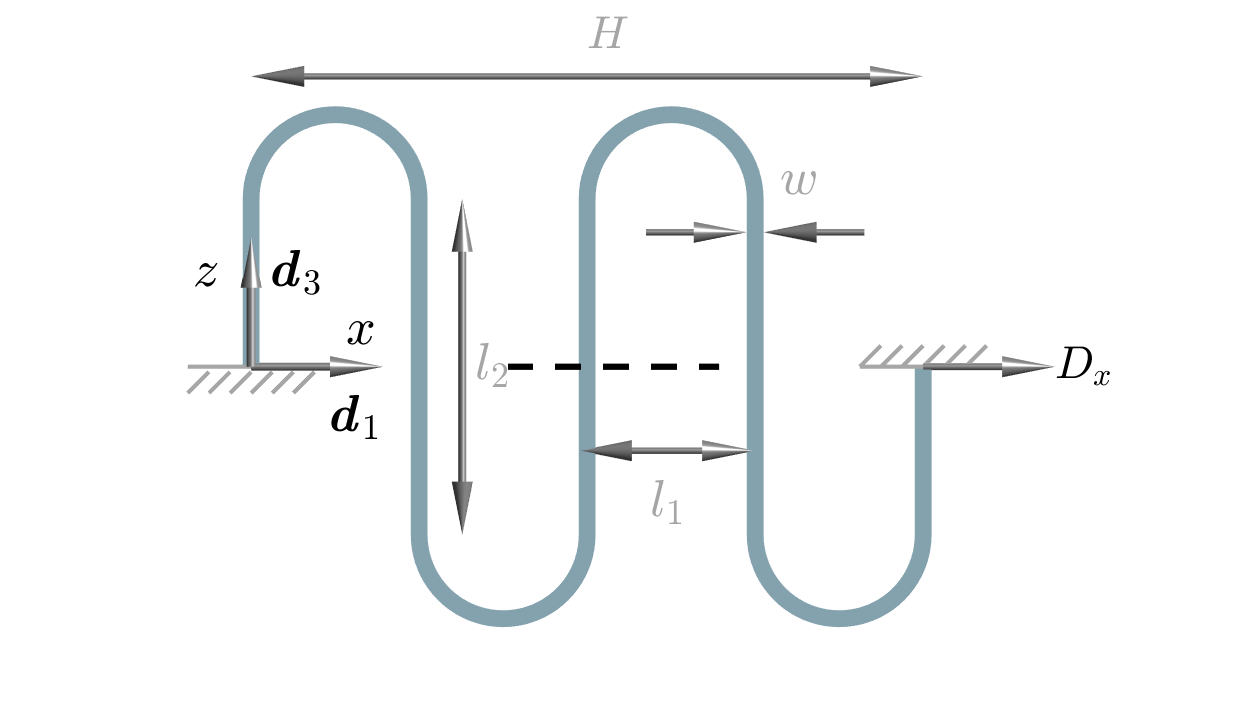
\includegraphics[width=0.6\linewidth]{Serpentine_Schematics}
	\caption{未变形时的双单元蛇形条带}
	\label{fig:Serpentine_Schematics}
\end{figure}

下面介绍如何用基尔霍夫杆模型来建立蛇形条带的力学模型。直线段与圆弧段的连接处的面内曲率不连续(圆弧段曲率为一个非零常数,而直线曲率保持为零),而基尔霍夫杆模型要求杆的曲率连续。因此需要在蛇形条带曲率不连续的地方进行分段,分别为每段条带建模并通过相应的连接条件将段与段之间相互连接。对于每一分段,根据式\eqref{eq:ToTle Equation}给出其控制方程。该方程中需要确定三个参数,分别为杆的长度$l$以及初始Darboux向量在材料坐标系$d_1$,$d_2$方向的分量$\kappa_{10}$,$\kappa_{20}$。对于杆长,这里将半圆弧段的条带长度设为1,作为单位来对其他分段长度进行无量纲化。设无量纲的结构高度为$\alpha$,那么一个单元中第一直线段与最后直线段的长度$l=\alpha/\pi$,中间直线段长度$l$为$2\alpha/\pi$。所有直线段的初始Darboux向量分量均为零。上半圆弧的Darboux向量的分量为$\kappa_{10}=0$,$\kappa_{20}=1/\pi$,而下半圆弧的Barboux向量对应的分量为$\kappa_{10}=0$,$\kappa_{20}=-1/\pi$。

对于单单元蛇形结构($n_c=1$)而言,共有五小段,每一分段可列$14$个控制方程,总共有$70$个微分方程。为了求解该微分方程,需要给出相同数量的边界条件。由初始端的固支约束可给出七个边界条件
\begin{equation}
	\begin{gathered}
	x^1(0)=0;\quad y^1(0)=0;\quad z^1(0)=0\\
	q^1_1(0)=1;\quad q^1_2(0)=0;\quad q^1_3(0)=0;\quad q^1_4(0)=0
\end{gathered}
\end{equation}
式中上标表示变量所属的条带分段,本处表示第一段上的变量。前三个边界条件固定条带初始端的位置,与四元数有关的四个条件用来固定转角。而对于整个结构的末端,同样可以根据固支条件施加七个边界条件
\begin{equation}
	\begin{gathered}
		x^5(1)=(1+p)\times\left(\alpha\cdot\frac{4}{\pi}\right);\quad y^5(1)=0;\quad z^5(1)=0\\
		q^5_1(1)=1;\quad q^5_2(1)=0;\quad q^5_3(1)=0;\quad q^5_4(1)=0
	\end{gathered}
\end{equation}
$p$为无量纲化的拉伸位移载荷。

另外,还需要给出分段与分段之间的连接条件
\begin{equation}
	\begin{gathered}
		N^i_1(0)=N^{i-1}_1(1);\quad N^i_2(0)=N^{i-1}_2(1);\quad N^i_3(0)=N^{i-1}_3(1)\\
		\kappa^i_{1}(0)=\kappa^{i-1}_{1}(1);\quad \kappa^i_{2}(0)-\kappa^i_{20}(0)=\kappa^{i-1}_{2}(1)-\kappa^{i-1}_{20}(1)\\
		\tau^{i}(0)=\tau^{i-1}(1) \quad \mathbfit{q}^{i}(0)=\mathbfit{q}^{i-1}(1) \quad \mu^{i}(0)=\mu^{i-1}(1)\\
		x^i(0)=x^{i-1}(1);\quad y^i(0)=y^{i-1}(1);\quad z^i(0)=z^{i-1}(1)
	\end{gathered}
\end{equation}
上式中,在每一连接处给出了十四个连接条件。式中上标$i$代表第$i$段条带上方程的变量,$i$可以取$2$,$3$,$4$,$5$。函数变量$0$为条带的首端,$1$为条件的末端。前三个边界条件为力的连续性条件。第三到第六个等式代表力矩的连续性条件。第七个式子为转角连续条件,第八个式子为常变量$\mu$的连续条件。最后三个式子代表位移连续条件。一个单元的蛇形条带有四个连接点,每个连接点处可以给出十四个连续性条件,外加十四个两端的固支边界条件,共有七十个边界条件。因此,结合方程与边界条件,可以组成一个适定的两点边界值问题。对于多单元的蛇形条带,只需要分别列出控制方程并在单元与单元之间给出相应的连接条件即可。

\subsection{弹性蛇形条带的实验}
本文对蛇形条带的研究,除了数值计算外,还通过实验来对数值结果进行验证。本小节简要介绍实验所用的加载装置以及蛇形条带的实物样本。
\begin{figure}
	\centering
	\includegraphics[width=1\linewidth]{ExptSetup (1).pdf}
	\caption{实验加载装置}
	\label{fig:ExptSetup}
\end{figure}

加载装置如图~\ref{fig:ExptSetup}所示,该装置通过SolidWorks设计三维模型并利用3D打印技术制作实物,所使用的3D打印机的型号为Creality Ender-3 S1如图~\ref{fig:3Dprinter}。加载装置主要由三部分组成:三个脚架,滑槽以及夹持结构。脚架的主要目的包括:(1)为整个结构提供支撑,(2)在滑槽下方预留适当的缝隙以容纳滑槽与加持结构之间的固定螺钉的延伸端。滑槽总长为\SI{50}{cm},由于3D打印机的成型尺寸限制,该滑槽被分为三个独立段进行加工,各滑槽之间铆接在一起,并通过螺钉固定以保证滑槽的稳定性。为便于拉伸位移的测量,滑槽上表面贴有刻度尺。夹持系统由两个加持臂构成。左侧加持臂固定于滑槽起始端,用以实现条带初始端的固支边界条件。右侧夹持臂具备轴向移动功能,可沿滑槽导轨平移,用于施加位移载荷。夹持臂的设计具有以下特征:(1)底部设有标准螺钉孔,可与滑槽狭缝配合实现位置锁定。(2)加持臂最上方设计有夹具,蛇形条带的末端可放入该夹具狭缝并通过两个上下排布的螺钉夹紧固定。在蛇形条带首末两端延伸出两个长方形末梢,如图~\ref{fig:ExptSetup}中深蓝色蛇形条带所示,用来将蛇形条带固定于夹具上。考虑到蛇形条带末梢的高度不同(左低右高),为了适应不同高度的加持末梢,在设计加持臂时,左右加持臂的高度不同(左低右高),左侧加持臂高度为\SI{20.5}{cm},右侧加持臂高度为\SI{23}{cm}。
\begin{figure}
	\centering
	\subcaptionbox{3D打印机\label{fig:3Dprinter}}
	{\includegraphics[width=0.4\linewidth]{3Dprinter.JPG}}
	\subcaptionbox{激光切割仪\label{fig:Laster Cutting}}
	{\includegraphics[width=0.4\linewidth]{Laster Cutting.JPG}}
	\caption{实验所用设备}
	\label{fig:experimental device}
\end{figure}

如图~\ref{fig:ExptSetup}所示,在图左侧,实验装置中设置了两个对比状态:不透明夹具上蛇形条带为初始未加载构型,而半透明夹具上条带为拉伸载荷作用下的屈曲构型。
\begin{figure}
	\centering
	\subcaptionbox{$\alpha=1.5$,$n_c=1$\label{fig:Serpentine Sample1.5}}
	{\includegraphics[width=0.11\linewidth]{Serpentine Sample1.5.pdf}}
	\subcaptionbox{$\alpha=4$,$n_c=1$\label{fig:Serpentine Sample4}}
	{\includegraphics[width=0.11\linewidth]{Serpentine Sample4.pdf}}
	\subcaptionbox{$\alpha=3$,$n_c=2$\label{fig:2Serpentine Sample3}}
	{\includegraphics[width=0.23\linewidth]{2Serpentine Sample3.pdf}}
    \subcaptionbox{$\alpha=3$,$n_c=3$\label{fig:3Serpentine Sample3}}
    {\includegraphics[width=0.36\linewidth]{3Serpentine Sample3.pdf}}
	\caption{蛇形条带实物}
	\label{fig:Samples of serpentine}
\end{figure}

图~\ref{fig:Samples of serpentine}展示了四个具有不同单元个数和高度的蛇形结构。这些蛇形结构通过AutoCAD设计,并利用激光切割仪(型号为Epilog FusionEdge,如图~\ref{fig:Laster Cutting}所示)在PVC塑料板上切割出相应的蛇形条带。所有蛇形结构的实际厚度为$t=\SI{0.24}{mm}$,截面宽度为$w=\SI{2.4}{mm}$(保证宽厚比为10)。同时将半圆弧直径设计条带宽度的十倍($R=5w$),即$2R=\SI{24}{mm}$,以保证蛇形结构的细长特性以及细长杆模型的有效性。若半圆弧直径小于截面宽度的十倍,那么二维的弹性理论\cite{wang2023substantial,yang2017elasticity}更适合捕捉此类结构的非线性特性,本文只考虑蛇形结构在细长情况下的力学行为。根据无量纲化高度$\alpha$以及半圆弧直径,可以得到实际的结构高度。$\alpha=1.5$对应的结构高度为$l_2=\SI{36}{mm}$,$\alpha=4$对应的结构高度为$l_2=\SI{96}{mm}$,$\alpha=3$对应的结构高度为$l_2=\SI{72}{mm}$。


\section{单单元蛇形条带分岔分析}
由于平面外弯曲刚度远小于平面内弯曲刚度,蛇形结构在拉伸载荷下会发生面外屈曲。Zhang等\cite{zhang2013buckling}在对蛇形结构的研究中发现,对于单单元蛇形条带($n_c=1$),其一阶屈曲模态的空间构形与结构的高度$\alpha$有关,具体而言,对于$\alpha<2.4$时,其一阶屈曲模态构形的俯视图展现出了反对称性,如图~\ref{fig:S_Mode}所示,由于其形状类似于字母S,下文称该模态为S模态;对于$\alpha>2.4$时,其一阶屈曲模态构形的俯视图展现出了正对称性,如图~\ref{fig:M_Mode}所示,下文称该模态为M模态。
\begin{figure}
	\centering
	\subcaptionbox{S模态\label{fig:S_Mode}}
	{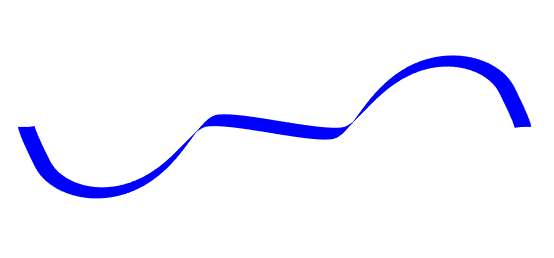
\includegraphics[width=0.3\linewidth]{S_Mode.eps}}
	\subcaptionbox{M模态\label{fig:M_Mode}}
	{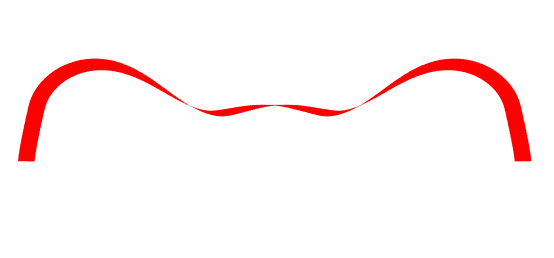
\includegraphics[width=0.3\linewidth]{M_Mode.eps}}
	\caption{单单元蛇形结构的一阶二阶屈曲模态}
	\label{fig:SM_Mode}
\end{figure}
针对这两类典型的蛇形结构,下面分别计算高度$\alpha=1.5$(代表一阶屈曲模态为S模态)以及高度$\alpha=4$(代表一阶屈曲模态为M模态)的单单元蛇形条带的分岔图,如图~\ref{fig:SerpentineNc1Aniso10}所示。

图~\ref{fig:SerpentineNc1Aniso10}(a-b),(d-e)分别为$\alpha=1.5$与$\alpha=4$的分岔图及其局部放大图。分岔图的横坐标对应于无量纲的位移载荷,纵坐标为图~~\ref{fig:SerpentineNc1Aniso10}(a)中蛇形结构上标记点$y_0$在拉伸载荷下的$y$方向位移。
从初始构形$D_x/H=0$出发,在结构的右端施加拉伸位移, 随着拉伸位移的增加,蛇形结构会发生面外屈曲使得原来的平面分支失稳(对应于$y_0=0$)。对于图~\ref{fig:SerpentineNc1Aniso10}(a)中$\alpha=1.5$的蛇形结构,在超临界分岔点$B_1$处,该结构发生屈曲,屈曲构形为一对稳定的S模态,(图~\ref{fig:SerpentineNc1Aniso10}(b)给出了该分岔点$B_1$处的放大图)。这一对S模态对应的两条平衡分支在超临界分岔点$B_3$后失稳,但在另一超临界分岔点$B_4$之后,该平衡分支重新稳定。在分岔点$B_4$之后,上下对称的一对S模态(对应图~\ref{fig:SerpentineNc1Aniso10}(c)中\bluesquare~/~\redsquare)始终保持稳定。除数值计算结果外,实验结果也表明:S模态除了在区间$B_3$,$B_4$之内,在其余位移载荷下均保持稳定。由分岔点$B_3$分岔得到的平衡分岔支与由分岔点$B_4$分岔出的平衡分支形成一个闭合的环,该闭合环上对应的模态(对应图~\ref{fig:SerpentineNc1Aniso10}(c)中\Brighttriangle~/~\Rrighttriangle~/~\Blefttriangle~/~\Rlefttriangle~)始终保持稳定,另外,该模态的空间构形并不具有对称性。在距分岔点$B_1$很近的后方,二次分岔点$B_2$出现并从该分岔点处分岔出一对平衡分支。该平衡分支在初始阶段其分支解为非稳定解,但在穿过亚临界分岔点$B_5$(考虑到分岔图的简洁性,这里没有展示从分岔点$B_5$分岔出的不稳定分支)之后,整个平衡分支变为稳定解,该稳定解为M模态(对应图~\ref{fig:SerpentineNc1Aniso10}(c)中~\Btriangle~/~\Rtriangle)。下面简要总结该蛇形结构在载荷不断增大时的行为,对于$\alpha=1.5$的蛇形条带,当位移载荷增大到分岔点$B_1$处,结构发生面外屈曲,屈曲模态为$S$模态。随着载荷进一步增加,原$S$模态在经过分岔点$B_3$之后,具有反对称特性的$S$模态分支失稳,结构沿$B_3$处分岔支变形(对应图~\ref{fig:SerpentineNc1Aniso10}(c)中\Brighttriangle~/~\Rrighttriangle~/~\Blefttriangle~/~\Rlefttriangle~),屈曲构形失去对称性。最后,进一步增大拉伸载荷,在经过分岔点$B_5$之后,构形又回到S模态对应的分支上并一直沿该分支变形上。
\begin{figure}[t]
	\centering
	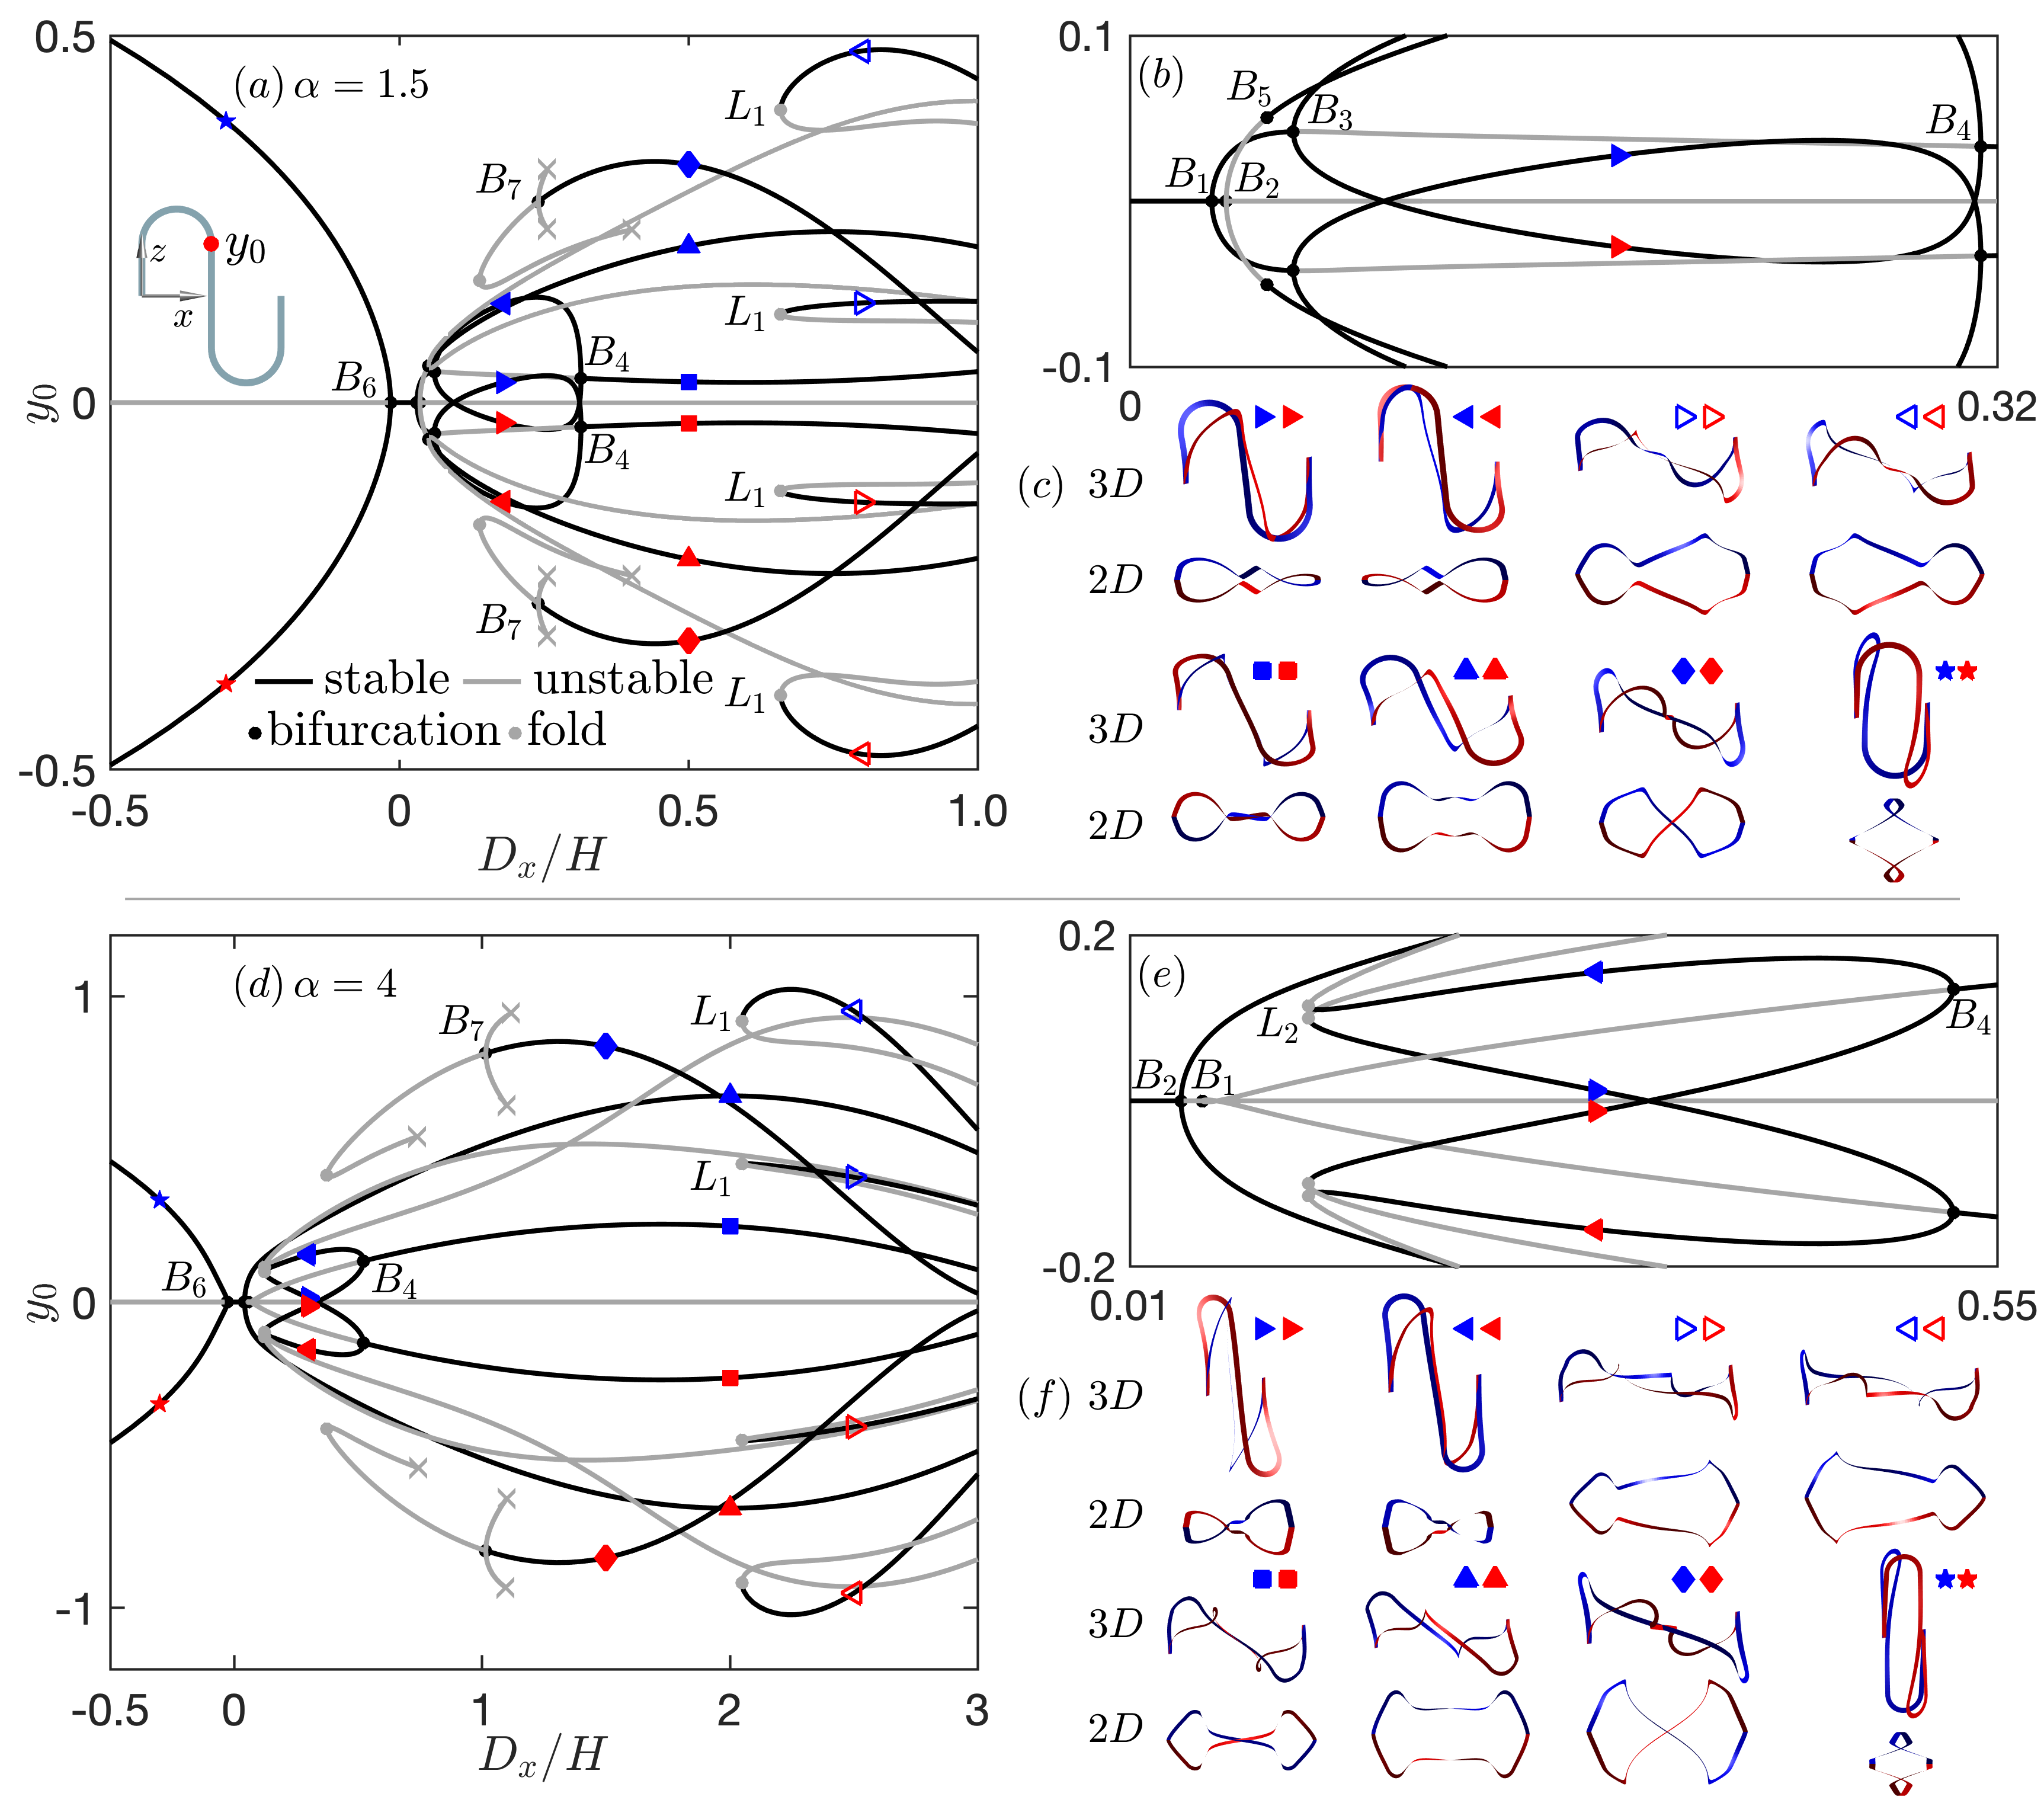
\includegraphics[width=1\linewidth]{SerpentineNc1Aniso10.png}
	\caption{不同高度的单单元蛇形结构的分岔图及对应分岔支的平衡构形。(a) $\alpha=1.5$的分岔图。(b) 图(a)的局部放大图。(c) 分岔图(a)中平衡分支对应的稳定构形。(d)  $\alpha=4$的分岔图。(e) 图(d)的局部放大图。(f) 分岔图(d)中平衡分支对应的稳定构形。}
	\label{fig:SerpentineNc1Aniso10}
\end{figure}

分岔图~\ref{fig:SerpentineNc1Aniso10}(a)中存在不与平面平衡分支$y_0=0$连接的其他稳定分支。其中一对这类孤立的分支为图~\ref{fig:SerpentineNc1Aniso10}(a)中(~\Rdiamond~/~\Bdiamond)中所标记的分支,该分支对应的解在亚临界分岔点$B_7$之后变为稳定解,该分支对应的构形同样为反对称构形(从俯视图观察)。另外,图~\ref{fig:SerpentineNc1Aniso10}(a)中\HBrighttriangle~/~\HRrighttriangle~/~\HBlefttriangle~/~\HRlefttriangle~标记的平衡分支同样不与平面解($y_0=0$)相连,且每一分支中存在一拐点$L_1$,意味着这些分支对应的稳定构形只有当载荷大于拐点$L_1$所对应的载荷才存在。在压缩位移载荷下($D_x/H<0$),蛇形结构同样会发生面外屈曲,当压缩位移超过超临界分岔点$B_6$时,蛇形结构发生面外屈曲,其屈曲模态为图~\ref{fig:SerpentineNc1Aniso10}(c)中~\Bstarshape~/~\Rstarshape。

图~\ref{fig:SerpentineNc1Aniso10}(d-e)为$\alpha=4$的蛇形结构的分岔图。相比于$\alpha=1.5$的分岔图,$\alpha=4$的分岔图中分岔点$B_1$和$B_2$的位置发生了交换,即分岔点$B_2$对应的载荷小于分岔点$B_1$对应的载荷,意味着随着载荷的增大,该蛇形结构会发生屈曲且其屈曲模态为一对M模态(对应图~\ref{fig:SerpentineNc1Aniso10}(f)中~\Btriangle~/~\Rtriangle~),而且该模态对应的分支解总为稳定解。分岔点$B_1$位于$B_2$之后不远处,从分岔点$B_1$分岔出的一对平衡分支在一开始为不稳定解,但经过超临界分岔点$B_4$之后,该分岔点变为稳定性解,对应着S模态(如图~\ref{fig:SerpentineNc1Aniso10}(f)中~\bluesquare~/~\redsquare~ 所示)。从分岔点$B_4$分岔出去的平衡分支(相应的稳定构形如图~\ref{fig:SerpentineNc1Aniso10}(f)中~\Brighttriangle~/~\Rrighttriangle~/~\Blefttriangle~/~\Rlefttriangle~所示),在一开始为稳定解,但经过拐点$L_2$之后该解失稳。在实际加载过程中,$\alpha=4$的蛇形条带在加载过程中,经过分岔点$B_2$之后,结构屈曲到M模态,并且在随后的加载过程中一直保持M模态。

类似于$\alpha=1.5$的蛇形结构,在$\alpha=4$的结构分岔图中同样存在不与平面平衡分支($y_0=0$)相连的解,包括一对上下对称的孤立分支,对应于图~\ref{fig:SerpentineNc1Aniso10}(f)中(~\Rdiamond~/~\Bdiamond)的构形,该分支对应的解在亚临界分岔点$B_7$之后变为稳定解。另外,图~\ref{fig:SerpentineNc1Aniso10}(c)中\HBrighttriangle~/~\HRrighttriangle~/~\HBlefttriangle~/~\HRlefttriangle~对应的平衡分支同样不与平面解对应的分支相连,且每一分支中存在一拐点$L_1$,意味着这些分支对应的稳定构形只有当载荷大于拐点$L_1$时对应的载荷才存在。

上述分析给出了两类典型高度的单单元蛇形结构的分岔图。Zhang等\cite{zhang2013buckling}发现当$\alpha<2.4$时,结构的屈曲模态为S模态,而当$\alpha>2.4$时,结构的屈曲模态为M模态。本节首先通过实验验证了同样的现象。随后,本文通过分岔分析对这一现象给出了解释:不论蛇形结构的高度,在足够的拉伸载荷下S模态和M模态均存在。但其出现的顺序不同,对于高度较小的蛇形结构,S模态出现所需的位移载荷小于M模态所需的载荷,即S模态为一阶屈曲模态,而M模态为二阶屈曲模态。而对于结构高度较大的蛇形条带,M模态为一阶屈曲模态,而S模态为二阶屈曲模态。

\section{多重特征值分岔}
上一节给出了两类典型高度的蛇形结构的分岔图,从图~\ref{fig:SerpentineNc1Aniso10}可以看到屈曲模态的交换对应于分岔点$B_1$,$B_2$的位置交换。另一方面,稳定性交换对屈曲模态的交换也至关重要。在$\alpha=1.5$的分岔图~\ref{fig:SerpentineNc1Aniso10}(a)中,一阶屈曲模态,即从$B_1$分岔点分岔出的平衡分支,在分岔点$B_1$附近为稳定解。二阶分岔点$B_2$分岔出的平衡分支在一开始为非稳定解。而对于$\alpha=4$的分岔图~\ref{fig:SerpentineNc1Aniso10}(d)具有相反的情况。从$B_1$分岔点分岔出的平衡分支,在分岔点$B_1$附近为非稳定解,分岔点$B_2$分岔出的平衡分支在一开始为稳定解。这种不同屈曲模态的稳定性交换,对屈曲模态交换至关重要,若不同分岔支上稳定性未发生交换,那么从分岔点$B_2$分岔出的分支为非稳定解,蛇形结构无法向非稳定分支延拓,因此不会屈曲为M模态,无法实现模态交换。本节将通过详细分析临界高度(不同模态交换刚好发生交换的高度)附近的分岔过程,揭示了不同屈曲模态对应分支的稳定性交换过程。
\begin{figure}
	\centering
	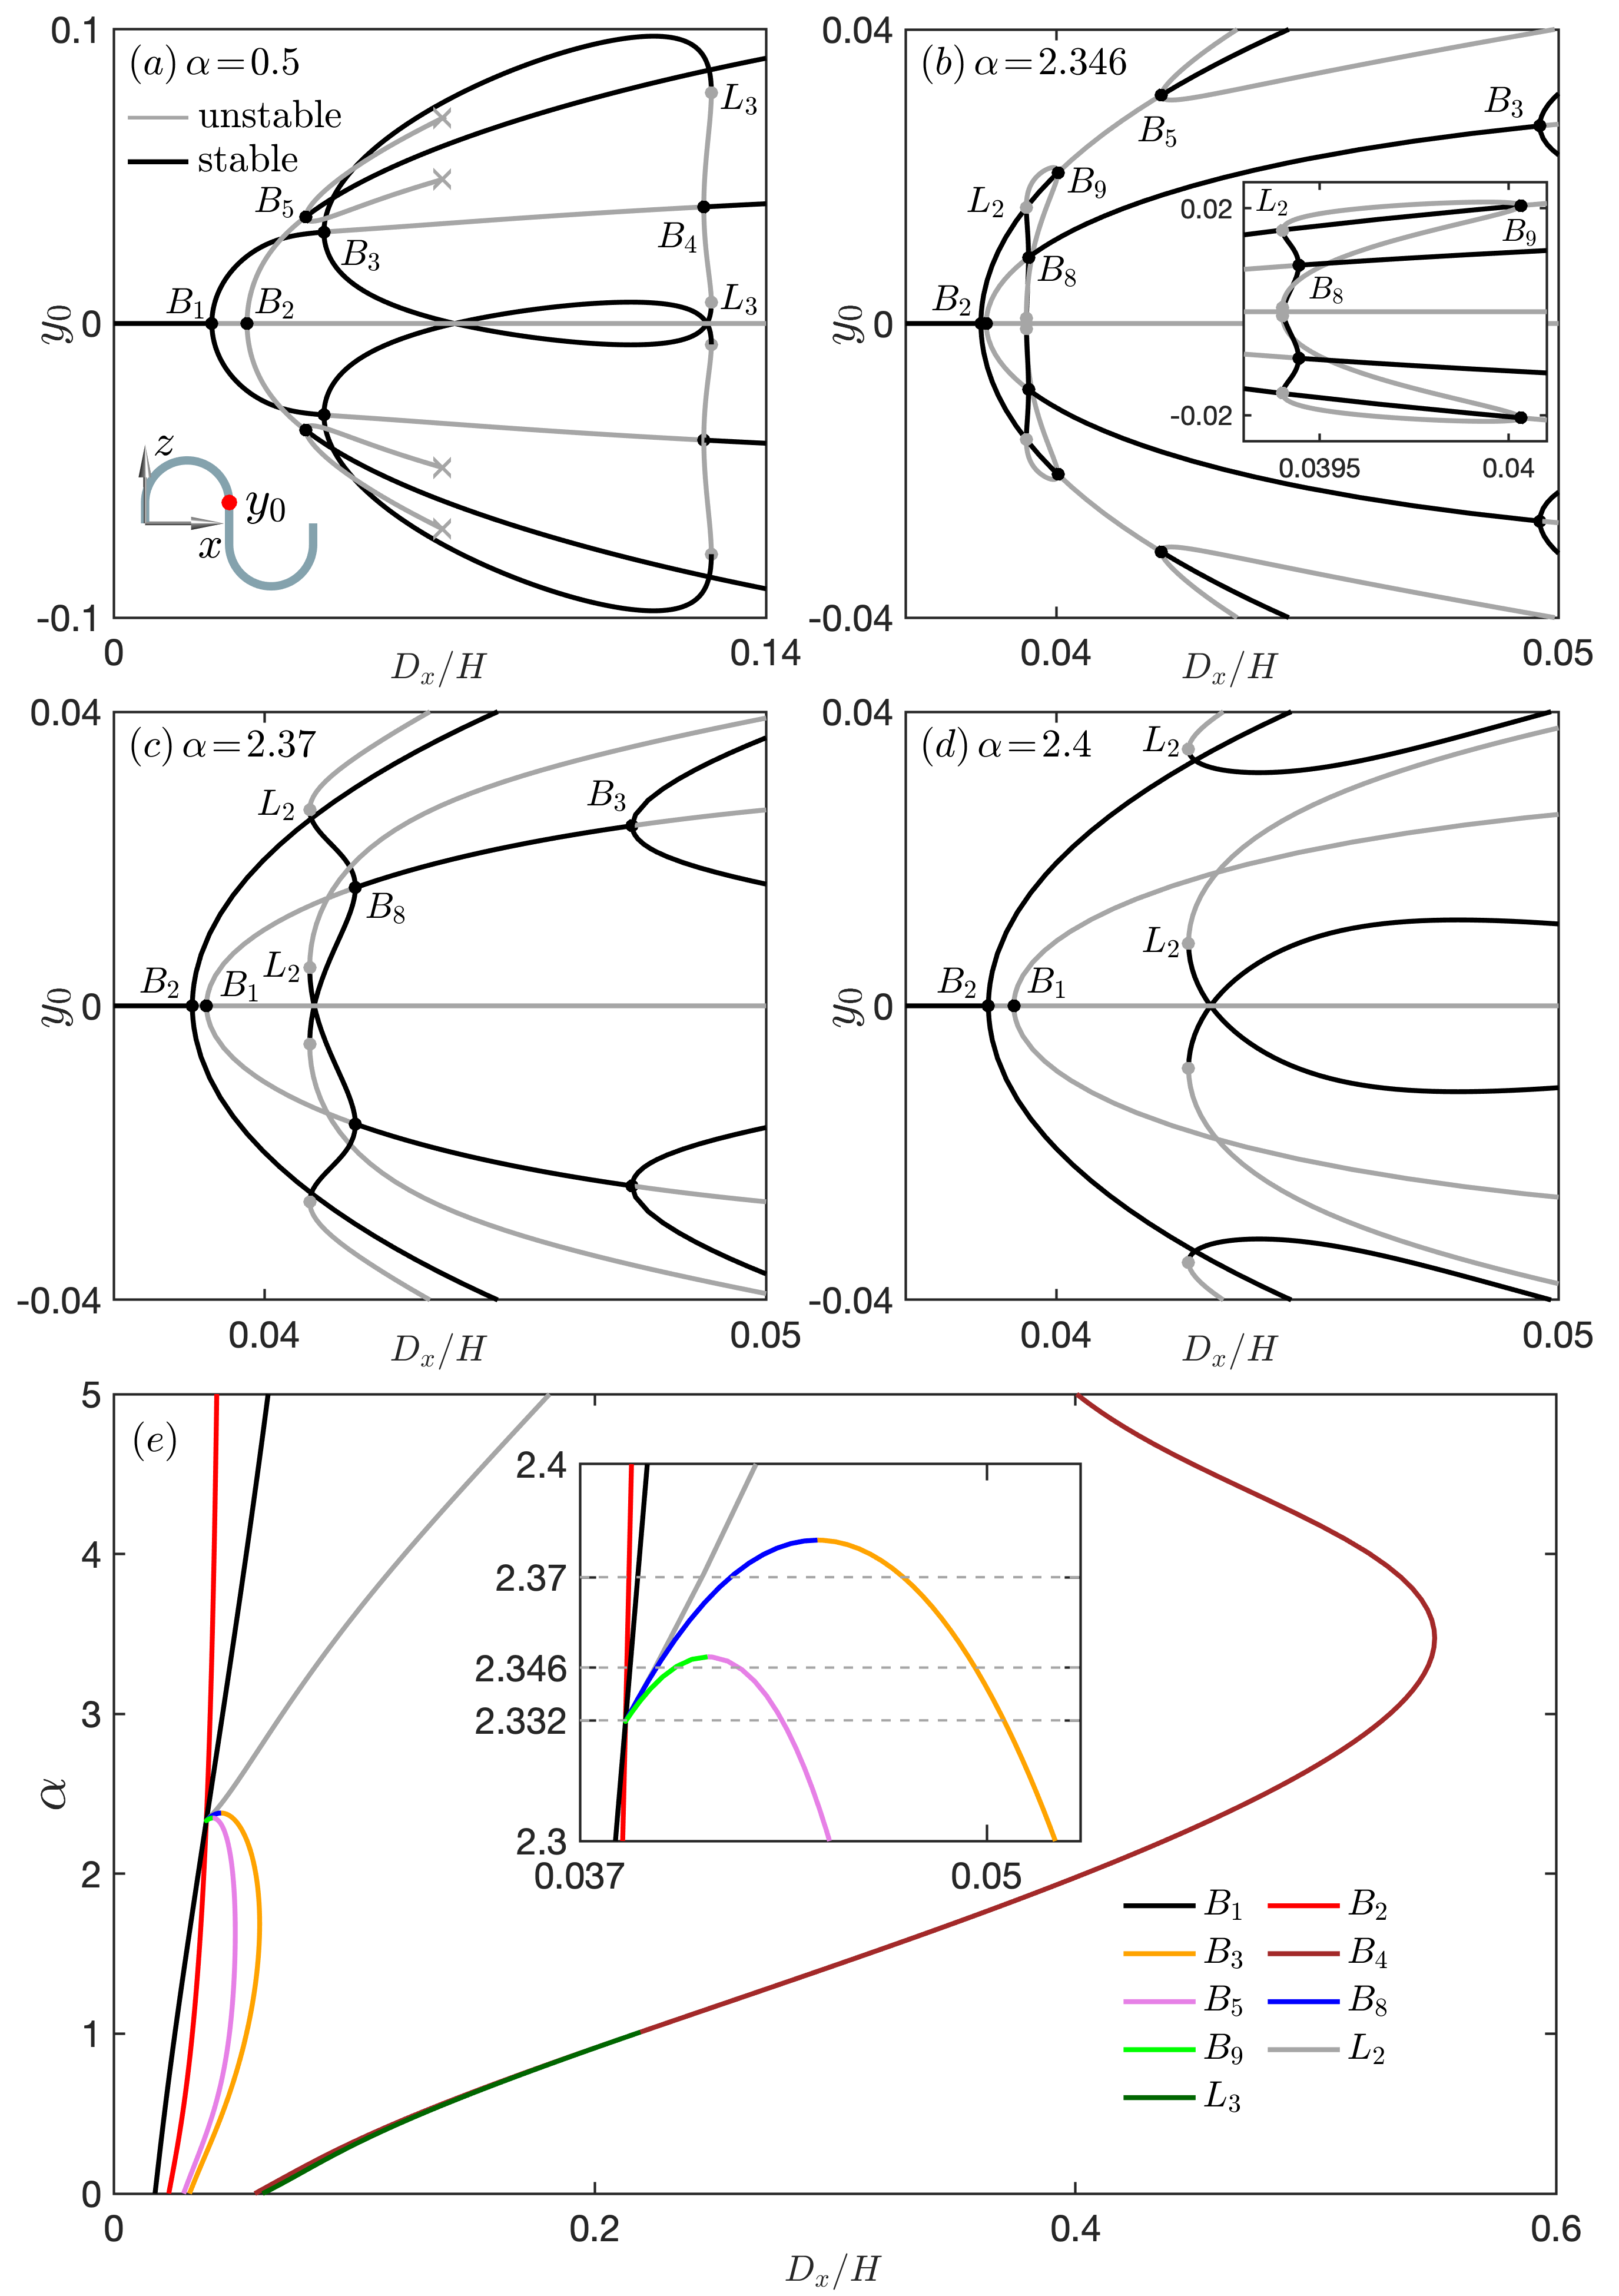
\includegraphics[width=1\linewidth]{SerpentineNc1Aniso10Phase.png}
	\caption{单单元蛇形条带不同屈曲模态交换的过程。(a-d) 不同高度$\alpha$下的分岔图。(e) 图(a-d)中分岔点随高度变化的轨迹。}
	\label{fig:SerpentineNc1Aniso10Phase}
\end{figure}

通过分岔分析软件AUTO 07P\cite{doedel2007auto}的双参数延拓功能可以计算绘制分岔点的轨迹曲线,图~\ref{fig:SerpentineNc1Aniso10Phase}(e)为分岔点的轨迹图,横坐标为相应分岔点的位置,纵坐标为无量纲的结构高度$\alpha$,图中黑色曲线为分岔点$B_1$随高度变化的轨迹,红色曲线为分岔点$B_2$沿高度变化的轨迹。在高度$\alpha=2.332$处时,两条轨迹线存在一交点,即分岔点$B_1$与分岔点$B_2$重合。该交点对应的高度为临界高度,高度大于该数值,结构在拉伸载荷下屈曲为M模态,低于该高度,结构会屈曲为S模态。该临界高度与Zhang等\cite{zhang2013buckling}所报道的$2.4$吻合。

在$\alpha=2.332$处,该系统为退化的情形,当$\alpha>2.332$时,两个二次分岔点$B_8$,$B_9$从$B_1$,$B_2$的交点处出现(对应于轨迹图~\ref{fig:SerpentineNc1Aniso10Phase}(e)的蓝色曲线和绿色曲线),为了更好地了解二次分岔点$B_8$,$B_9$的演化过程,本文绘制了$\alpha=2.346$下(对应于二次两个分岔点$B_8$,$B_9$同时存在的情形)的分岔曲线,如图~\ref{fig:SerpentineNc1Aniso10Phase}(b)所示。从图中可以看到二次分岔点$B_8$,$B_9$分别在$B_1$,$B_2$对应的分岔支上,$B_8$的出现使得$B_1$到$B_8$区间中原本稳定的平衡分支失稳,而$B_9$的出现使得$B_2$到$B_9$区间中原本不稳定的平衡分支获得稳定性。从轨迹图~\ref{fig:SerpentineNc1Aniso10Phase}(e)可以看出分岔点$B_8$,$B_9$从$B_1$,$B_2$的交点出发,分别逐渐向分岔点$B_3$,$B_5$靠近。随着$B_8$的靠近,$B_1$分岔出的平衡分支稳定区间($B_1$—$B_3$)逐渐失稳。而随着$B_9$的靠近,$B_2$分岔出的平衡分支非稳定区间($B_2$—$B_5$)对应的解逐渐变为稳定解。图~\ref{fig:SerpentineNc1Aniso10Phase}(b)只标记了$y_0>0$的二次分岔点,对于$y_0<0$的情况,同样也会存在相同的二次分岔点,上下两对分岔点$B_8$,$B_9$共同构成了一个闭合的环形分岔支。随着高度$\alpha$的减小,这个环形分岔支会逐渐缩小到最终与$B_1$,$B_2$的交点重合。

上述演化过程对应着一类典型的分岔行为——多重特征值分岔(double eigenvalue bifurcation),该分岔行为存在于各类力学现象中\cite{bauer1975multiple,tavener1988buckling,keener1979secondary}。当系统某一参数发生变化时,一个多重分岔点会分裂为两个主分岔点以及若干个二次分岔点\cite{bauer1975multiple}。在本文的情形中,$B_1$,$B_2$为主分岔点,$B_8$,$B_9$为二次分岔点。在$\alpha=2.332$下,$B_1$,$B_2$的交点处为多重特征值分岔点,随着$\alpha$增大,该多重特征值分岔点分裂为两个主分岔点$B_1$,$B_2$,以及两个二次分岔点$B_8$,$B_9$。而二次分岔点的出现促使不同分岔支发生稳定性交换。

从轨迹图~\ref{fig:SerpentineNc1Aniso10Phase}(e),当结构高度$\alpha$增加到某一数值之后,二次分岔点$B_9$与分岔点$B_5$融合(在某一高度处,绿色轨迹与紫色轨迹相连)。$\alpha=2.37$为融合之后的某一结构高度,其分岔图为~\ref{fig:SerpentineNc1Aniso10Phase}(c),图中可以看到分岔点$B_2$对应的分岔支上无二次分岔点$B_9$,$B_5$的出现,使得整个平衡分支对应稳定解。随着高度的进一步增加,二次分岔点$B_8$与分岔点$B_3$融合(在某一高度处,图~\ref{fig:SerpentineNc1Aniso10Phase}(e)中蓝色轨迹与橘色轨迹相连)。$\alpha=2.4$为融合之后的某一高度,其分岔图为~\ref{fig:SerpentineNc1Aniso10Phase}(d),图中可以看到分岔点$B_1$对应的分岔支上无二次分岔点$B_8$,$B_3$的出现,分岔点$B_1$分岔出的分支在分岔点$B_4$之前为非稳定解。
\section{多单元蛇形条带分岔行为}
前面两节对单单元蛇形结构进行了分岔分析并揭示了不同屈曲模态交换的数学机理。但在蛇形结构的实际应用中,多单元蛇形结构往往具有更广泛的应用场景。因此,本节考虑多单元蛇形结构的分岔行为,以$\alpha=3$,单元数$n_c=2$和$n_c=3$的蛇形结构为例进行分岔分析,类似的分析方法可以用于分析其余任意单元数,任意高度的蛇形结构。

图~\ref{fig:SerpentineNc2Nc3Aniso10Phase}给出了相应的数值计算结果。图~\ref{fig:SerpentineNc2Nc3Aniso10Phase}(a-d)分别展示了$n_c=2$,$\alpha=3$的分岔图,分岔图的局部放大图,分岔图中平衡分支对应的稳定构形,以及分岔图中分岔点随结构高度变化的轨迹图。类似于图~\ref{fig:SerpentineNc2Nc3Aniso10Phase}(a-d),图~\ref{fig:SerpentineNc2Nc3Aniso10Phase}(e-f)展示了$n_c=3$,$\alpha=3$的蛇形结构对应的数值计算结果。对于这两种不同单元数的情况,蛇形结构在经过超临界分岔点$B_1$之后会发生屈曲,其屈曲模态均为S模态(对应图~\ref{fig:SerpentineNc2Nc3Aniso10Phase}(c),(g)中~\Bdiamond~所标记的构形),分岔点$B_1$之后存在第二个分岔点$B_2$,从分岔点$B_2$分岔出的两个分岔支在初始时为不稳定的平衡解,但在该分支上存在一对(上下分支各一个)亚临界分岔点$B_3$,在该分岔点之后,从分岔点$B_2$分岔出的两个分支变为稳定平衡解,对应的平衡构形为图~\ref{fig:SerpentineNc2Nc3Aniso10Phase}(c),(f)中~\bluesquare~所标记的M模态。 图~\ref{fig:SerpentineNc2Nc3Aniso10Phase}(d),(h)为各个分岔点随高度$\alpha$变化的轨迹图,从图中可以看出,分岔点$B_1$的出现总是先于分岔点$B_2$,即分岔点$B_1$与分岔点$B_2$的轨迹在$\alpha \in \left[0 \, 5\right]$内无交点出现。这说明对于多单元蛇形条带而言,蛇形结构的一阶屈曲模态总为S模态,二阶屈曲模态总为M模态。这一结论与Zhang等\cite{zhang2013buckling}的结论:多单元结构的屈曲模态总为反对称模态(对应本文中的S模态)一致。除这两个屈曲模态外,多单元蛇形结构在后屈曲范围内,存在更多的稳定性状态,例如图~\ref{fig:SerpentineNc2Nc3Aniso10Phase}(a),(c)中存在以~\Btriangle(对应图~\ref{fig:SerpentineNc2Nc3Aniso10Phase}(c),(g)中~\Btriangle~所标记的构形)和$~\Bstarshape~$(对应图~\ref{fig:SerpentineNc2Nc3Aniso10Phase}(c),(g)中~\Bstarshape~所标记的构形)标记的不与平面解$y_0$相连的分支。~\Btriangle~标记的孤立分支在载荷大于拐点$l_1$时才会存在;而~\Bstarshape~标记的孤立分支在载荷大于拐点$l_2$时才会存在。

\begin{figure}[t]
	\centering
	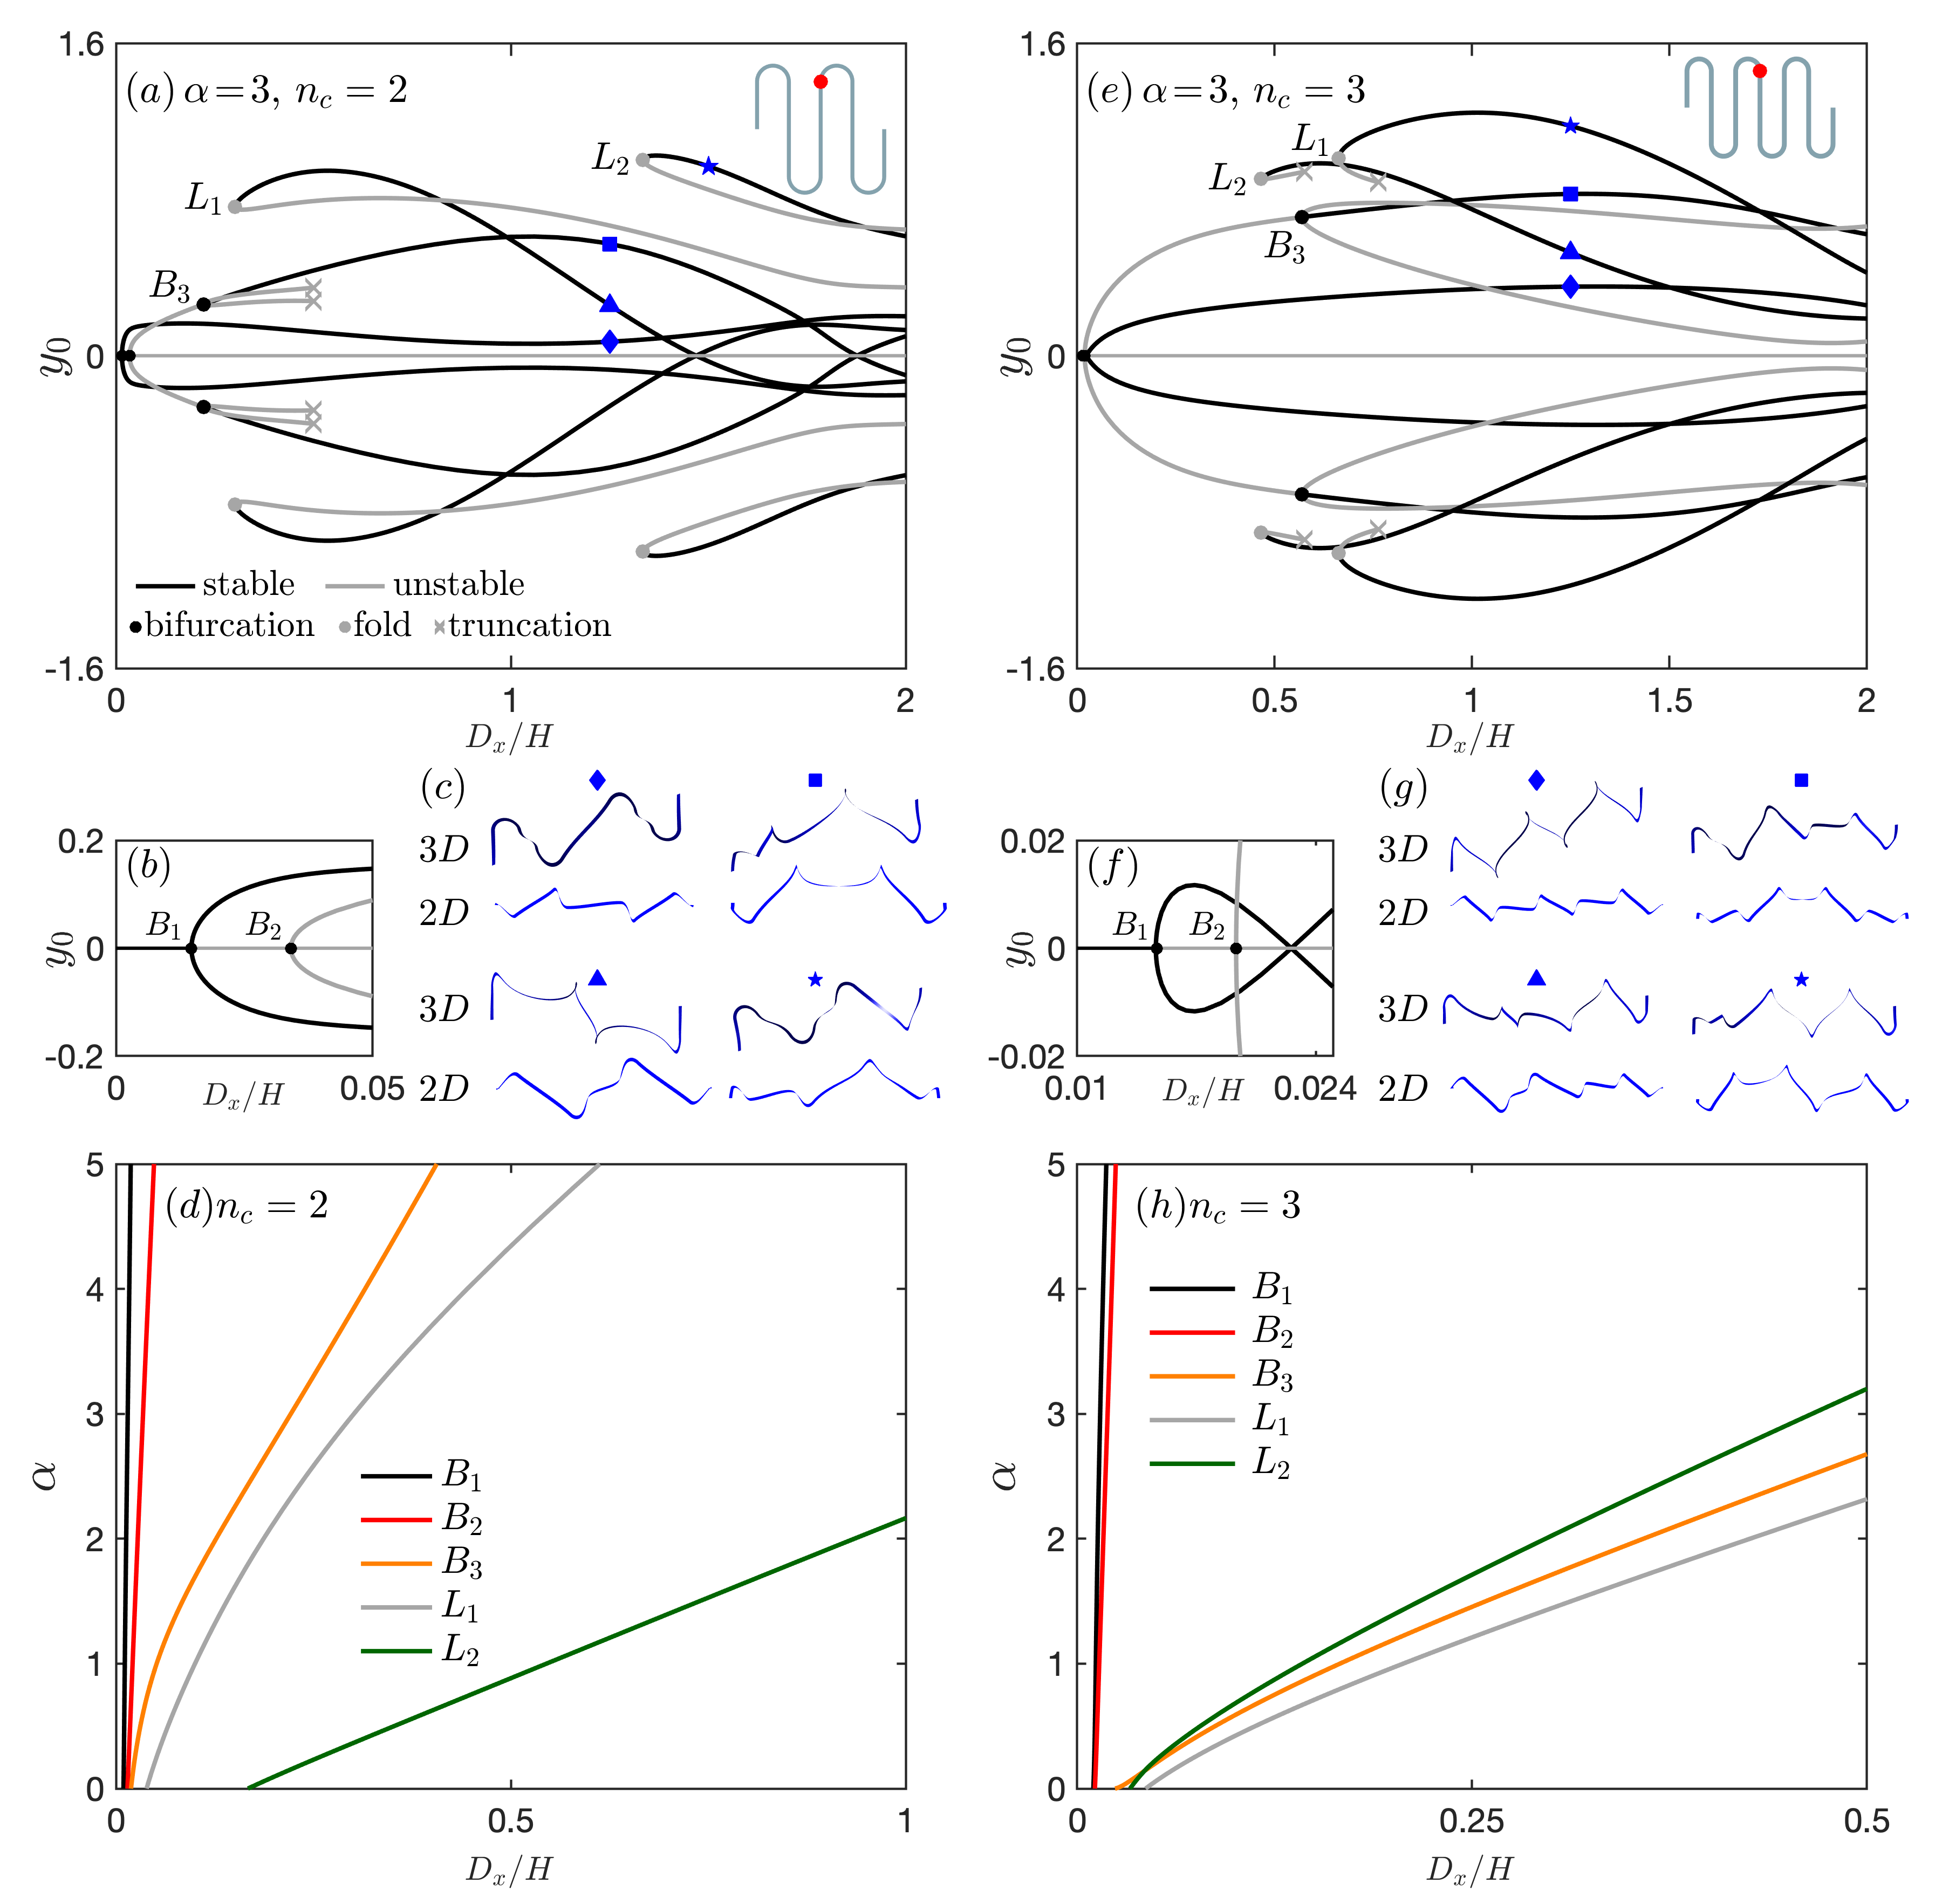
\includegraphics[width=1\linewidth]{SerpentineNc2Nc3Aniso10Phase.png}
	\caption{$n_c=2$,$n_c=3$的蛇形结构的分岔图及其相应分岔点的轨迹,$y_0$表示分岔图(a),(e)中蛇形结构红色标记点的平面外位移($y$方向)。(a) $n_c=2$,$\alpha=3$分岔图。(b) 图(a)的放大图。(c) 图(a)中平衡分支对应的构形。(d) 图(a-b)中分岔点的轨迹图。(e) $n_c=3$,$\alpha=3$分岔图。(f) 图(e)的放大图。(g) 图(e)中平衡分支对应的构形。(h) 图(e-f)中分岔点的轨迹图。}
	\label{fig:SerpentineNc2Nc3Aniso10Phase}
\end{figure}
\section{弹性蛇形条带的多稳态行为}
\subsection{稳态解的获得}
多稳态特性是蛇形结构的另一特点,在某一固定的水平拉伸位移载荷下,蛇形结构往往存在多个稳定的构形。本节通过数值模拟及实验的手段研究了单元数$n_c=1,2,3$的蛇形结构的多稳态行为。从以拉伸位移为延拓参数的分岔图~\ref{fig:SerpentineNc1Aniso10}和~\ref{fig:SerpentineNc2Nc3Aniso10Phase}中可以看出,一部分解与平面分支解$y_0=0$相连,如图~\ref{fig:SerpentineNc1Aniso10}(a),(d)中S模态(~\bluesquare~/~\redsquare~)与M模态(~\Btriangle~/~\Rtriangle~)等对应的平衡分支,为了获得这类解,可将未受拉伸的状态对应的解(力与力矩均为零,结构的空间构形已知)作为参数延拓的初始解。然而部分平衡分支并不与解$y_0=0$相连,如图~\ref{fig:SerpentineNc1Aniso10}(a),(d)和~\ref{fig:SerpentineNc2Nc3Aniso10Phase}(a),(e)中~\Bdiamond~/~\Bstarshape~所标记的平衡分支。对于此类解,无法直接从未受拉伸的解开始延拓得到,为了得到这些孤立平衡分支,需要已知这些孤立分支上的某一点的解作为启动解来获得整条平衡分支。

为了得到这些孤立分支上的一个启动解,一种方法是基于弹性杆静力学平衡方程的方法,通过延拓某一扰动载荷来建立不同的稳定分支之间的联系\cite{Arena_2018,arena2017adaptive}。具体而言,首先从未受载的状态开始,以目标载荷(蛇形条带中,为水平拉伸位移载荷)为延拓参数进行参数延拓,得到特定载荷下的某一稳定构形。然后固定此延拓参数,在该稳定构形上施加某种扰动外力并将该外力作为延拓参数进行延拓,若扰动外力选取得当,所得延拓曲线上存在若干扰动外力为零的点。每一外力为零的点代表着一个平衡解,这样就联系起了在某一固定拉伸载荷下的各个平衡分支。然而对于复杂结构,如蛇形结构,在扰动外力作用下,往往会产生一条复杂的延拓曲线,曲线上存在很多扰动外力为零的点。但这些外力为零的点对应的平衡解往往是非稳定解,无法得到期望的稳定平衡解。

本文采用一种更为有效的方法来寻找稳态解,类似于上述方法,该方法仍通过施加扰动外力的方法寻找稳态解。但不同于上述方法中使用静力学方程进行参数延拓,本方法采用动力学杆模型(这里采用离散弹性杆模型)来进行动力学模拟,在扰动外力下结构直接从某一平衡构形突跳到另一平衡构形。该方法相较于第一种方法具有如下优势:(1)动力学模拟可以捕捉结构的动力学过程,例如结构的突跳过程,使得结构可以直接从某一构形突跳到另一构形上。(2)动力学得到的扰动外力为零的平衡点一定对应稳定解,无需进行额外的稳定性判断。

本节通过下述四个加载过程使得结构从一个稳定构形跳变到另一稳定构形:
\begin{enumerate}
	\item 对结构施加水位移载荷使结构拉伸到目标长度,在阻尼力的作用下,结构会随时间趋于静力学平衡状态。
	\item 在所得稳定的平衡构形上施加扰动力(力矩),当扰动力(力矩)增加到某一临界值时,结构会发生突跳,切换到新的构形上。
	\item 撤除该扰动力,使结构逐渐恢复到未受扰动力的新平衡构形,该平衡构形为新的稳定解。
	\item 在新构形的基础上继续施加扰动,可以得到另一新的构形,如此反复,直到目标构形出现。
\end{enumerate}

对于扰动力(力矩)的确定,包括施加力的位置和具体力的形式(方向、大小),依赖于实验观察。通过实验观察可知,蛇形结构的多稳态表现为结构每一半圆弧段在足够的拉伸位移下,会表现出两种稳定的取向。在多单元蛇形结构中,由于半圆弧段数的增多,结构稳定构形随半圆弧段数增多而急剧增多。因此施加扰动的目的是切换半圆弧段的取向,在扰动力的作用下,半圆弧段从某一取向跳变到另一取向时,蛇形结构的其余部分会随着该切换过程移动到新的位置,达到新的稳态构形。根据实验可知,在半圆弧末端施加扭转力矩,力矩方向始终沿中心线切线方向,可以有效切换相应半圆弧段的取向。对于扰动力矩的大小,本文通过数值计算来确定,结构突跳发生时所需的最小力矩即为所需扰动力矩的大小。以一个双单元蛇形结构($n_c=2$,$\alpha=3$)的突跳为例,如图~\ref{fig:Disturb}所示。从反对称构形(S模态)开始在左起第一个半圆弧末端施加方向沿弧长切线方向的力矩后,该结构从深蓝色条带的构形突跳到半透明蓝色构形。
\begin{figure}
	\centering
	\includegraphics[width=1\linewidth]{Disturb.png}
	\caption{$n_c=2$,$\alpha=3$的蛇形结构在施加扰动前后的平衡构形。其中半透明条带为突跳后的构形,而深蓝色条带为突跳前的构形}
	\label{fig:Disturb}
\end{figure}
\subsection{蛇形条带平衡解的可逆对称性}
在研究蛇形结构的多稳态行为时,利用该结构的对称性可以有效简化分析过程。具体而言,若找到某一稳定平衡解,那么可以通过该结构的对称性直接推断出与其有对称关系的其他稳定平衡解,而无需针对每一稳定平衡解进行动力学模拟。因此,本小节重点研究蛇形结构的对称性。

细长条带结构在两端固支的条件下,往往表现出可逆对称性\cite{starostin2022forceless,van1998lock,champneys1996multiplicity,domokos2001hidden}(reversible symmetry),即同一边界值问题(BVP)的不同的解之间存在一定的关系。

蛇形结构在未加载时的构形呈现出了反对称性,即以结构的几何中心为旋转中心,以$y$轴为旋转轴,做旋转变换,旋转$180^\circ$后构形与原构形重合。因此,若已知某一屈曲构形,那么一定可以通过上述旋转变换,可以得到另外一个满足边界条件的构形。另外,若已知某一构形,那么一定可以通过以$x-z$平面做镜像对称得到另外一满足边界条件的构形。如图~\ref{fig:Groups with four configurations}所示,若在计算过程中得到第一个平衡构形,那么以该构形为基准,通过镜面对称可以得到第二个构形。将第二个构形旋转$180^\circ$可以得到第三个构形,接着对第三个构形进行镜面对称,可以得到第四个构形。因此若已知某一稳态构形,那么一定伴随着其他三个满足边界条件的构形的出现。但需要注意的是,若某一屈曲构形自身具有旋转对称性,那么通过镜面对称变换与通过旋转变换所得构形为同一构形。如图~\ref{fig:reversible pairs}所示,将最左侧构形进行旋转变换或者镜像对称,得到的构形均为第二个构形。因此,可以将蛇形条带的所有屈曲构形分为两类,一类构形本身具有旋转对称性,此类构形总是成对存在,下文将该构形对称为自可逆构形对,另外一类构形自身不具有旋转对称性,此类构形总是成组存在,每组中有四个构形,下文将该类构形组称为平衡构形组。例如,从图~\ref{fig:SerpentineNc1Aniso10}(c)(f)可以看出图~\ref{fig:SerpentineNc1Aniso10}(a)(d)中以~\Brighttriangle/~\Blefttriangle~/~\Rlefttriangle~/~\Rrighttriangle~所标记的四条平衡分支属于同一平衡构形组。以~\HBrighttriangle/~\HBlefttriangle~/~\HRlefttriangle~/~\HRrighttriangle~标记的平衡分支属于另一平衡构形组。以~\bluesquare/~\redsquare~标记的平衡分支属于同一自可逆对。以~\Btriangle/~\Rtriangle~标记的平衡分支属于另一自可逆对。
\begin{figure}
	\centering
	\subcaptionbox{$\alpha=3$,$n_c=2$的一个自可逆构形对\label{fig:reversible pairs}}
	{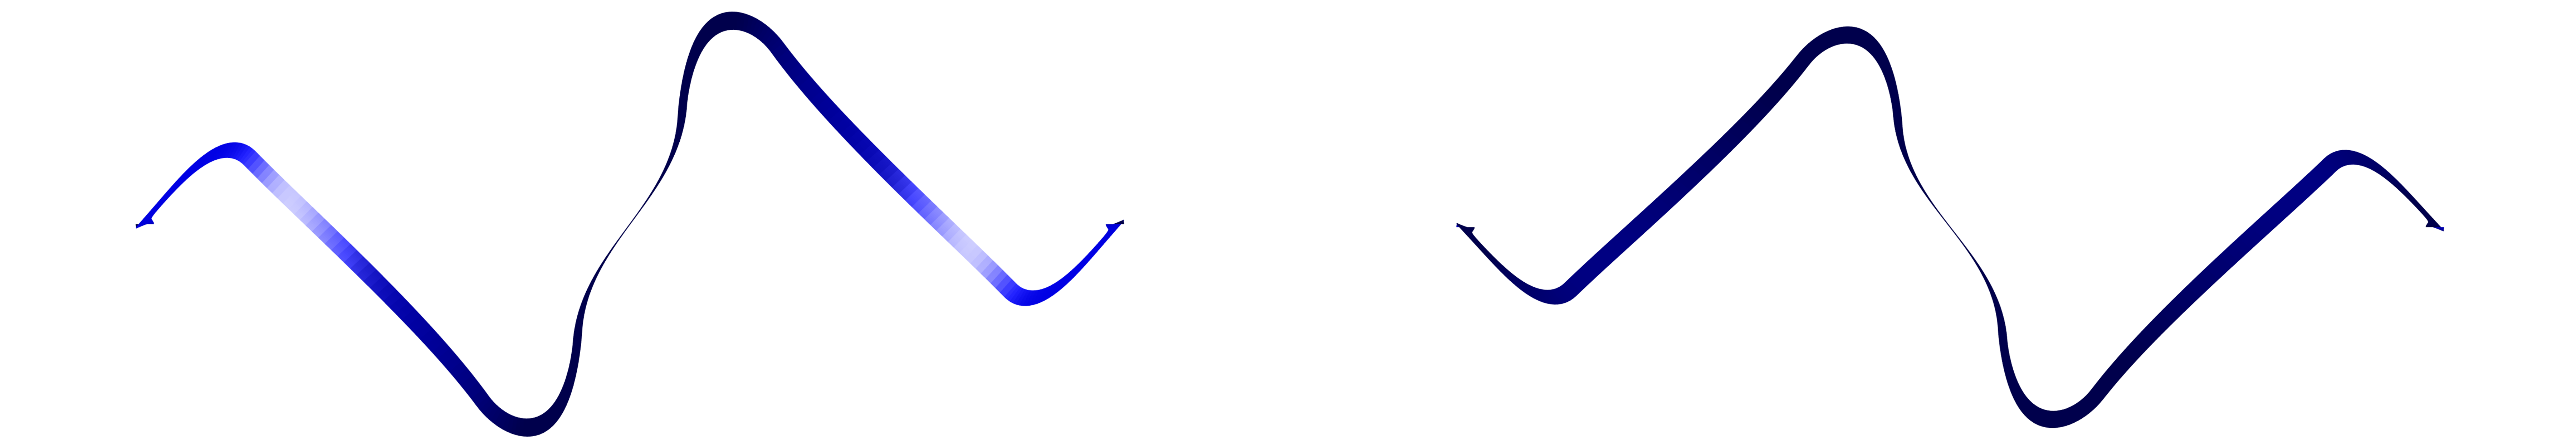
\includegraphics[width=0.45\linewidth]{reversible pairs.png}}\\
	\subcaptionbox{$\alpha=3$,$n_c=2$的一个平衡构形组\label{fig:Groups with four configurations}}
	{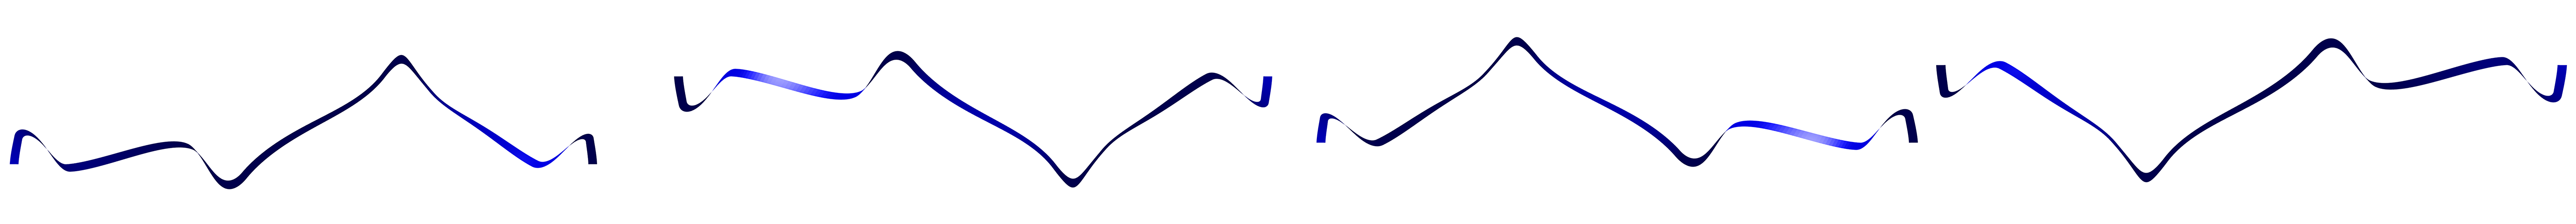
\includegraphics[width=1\linewidth]{Groups with four configurations.png}}
	\caption{$\alpha=3$,$n_c=2$的六个平衡构形}
	\label{fig:reversible pairs and group}
\end{figure}

为了寻找同一自可逆对或同一平衡构形组之内各构形解的关系,本文首先通过施加扰动外力的方法,得到某一平衡构形组(自可逆对)中的所有平衡解,然后观察该组解中各变量之间的变换关系。将所得变换关系代入微分方程来验证该变换关系对任一平衡构形组均有效。对于细长杆结构,若已知该杆的曲率,挠率以及杆内力的三个分量,那么可以唯一确定该弹性杆的构形以及受力情况。因此下面重点研究这六个关键变量之间的关系。

\begin{figure}
	\centering
	\subcaptionbox{~\bluesquare~:$\kappa_1,\kappa_2,\tau$曲线\label{fig:Ra}}
	{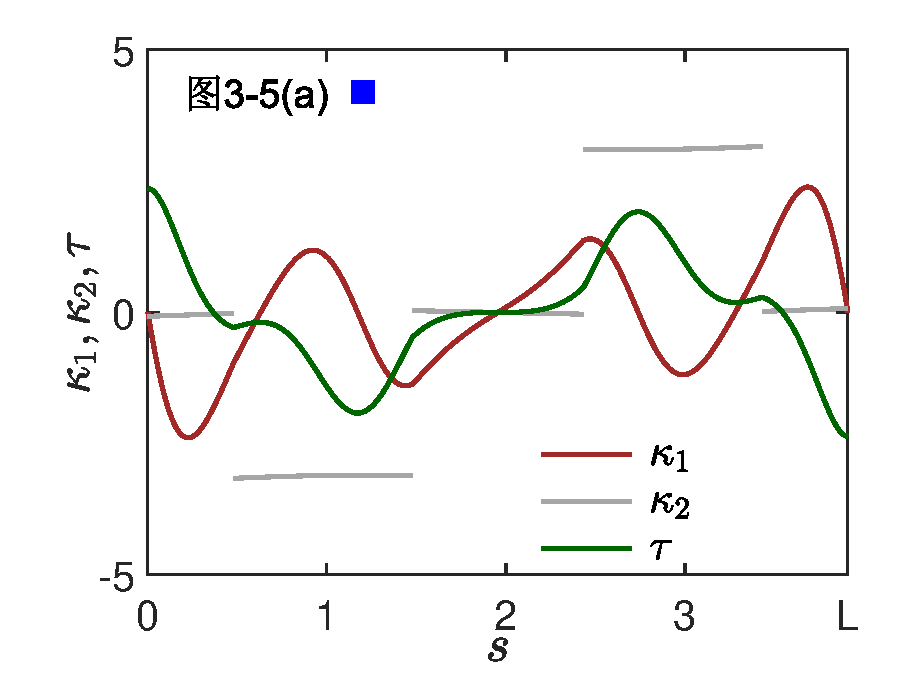
\includegraphics[width=0.45\linewidth]{Ra.eps}}
	\subcaptionbox{~\redsquare~:$\kappa_1,\kappa_2,\tau$曲线\label{fig:Rb}}
	{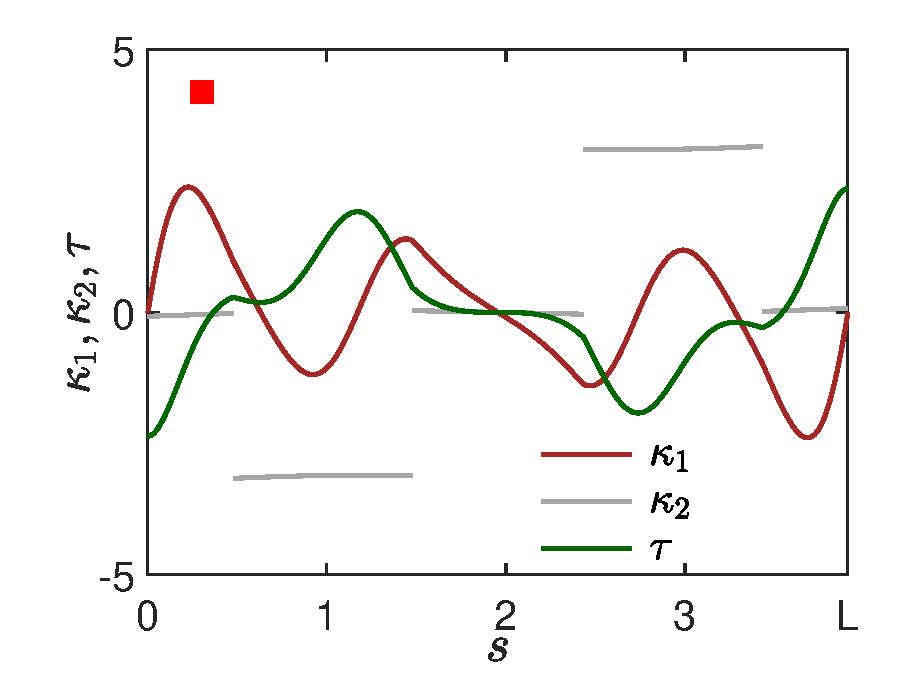
\includegraphics[width=0.45\linewidth]{Rb.eps}}\\
	\subcaptionbox{~\bluesquare~:$N_1,N_2,N_3$曲线\label{fig:R3}}
	{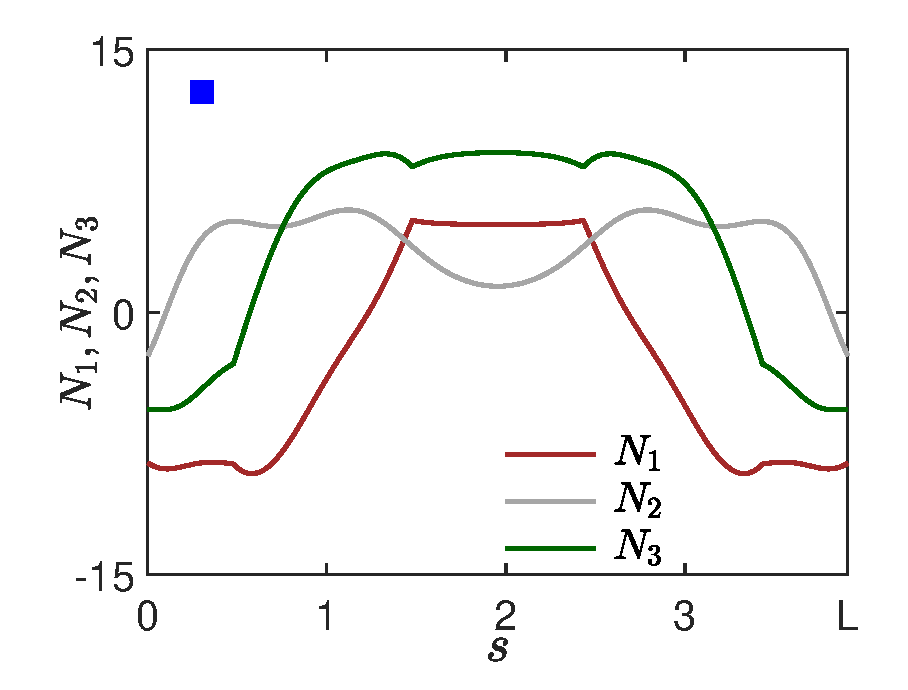
\includegraphics[width=0.45\linewidth]{R3.eps}}
	\subcaptionbox{~\redsquare~:$N_1,N_2,N_3$曲线 \label{fig:Rd}}
	{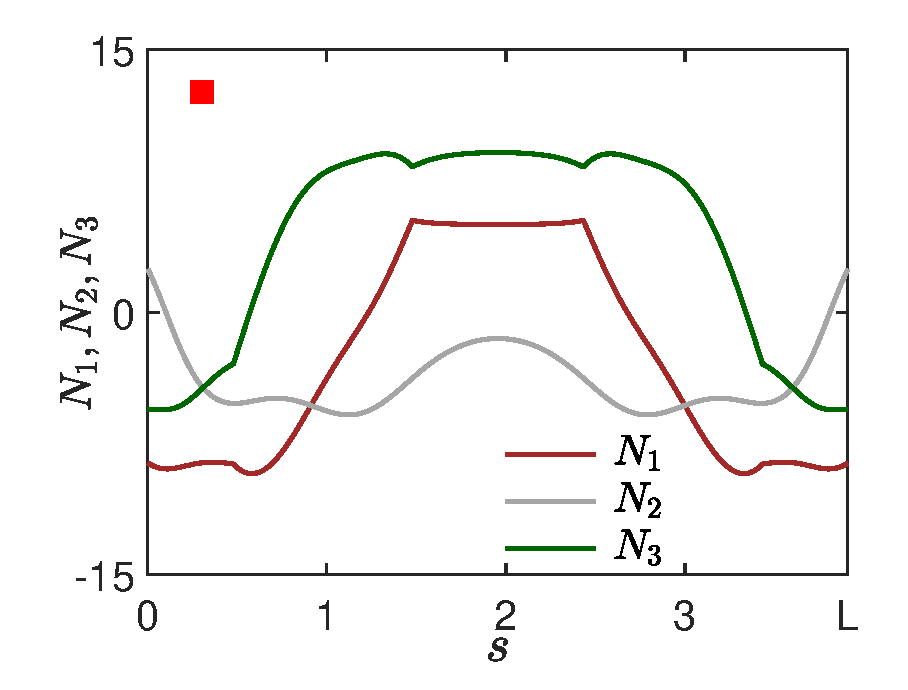
\includegraphics[width=0.45\linewidth]{Rd.eps}}
	\caption{图~\ref{fig:SerpentineNc1Aniso10}(c)中标记所对应构形的解曲线}
	\label{fig:relation in reversible pair}
\end{figure}
图~\ref{fig:relation in reversible pair}为$\alpha=1.5$,$n_c=1$的蛇形结构的两个互为镜像对称的S模态(共同构成了一个自可逆对)的解曲线,通过观察可知这六个变量具有如下关系:
\begin{equation}
	K: s \rightarrow s, \kappa_{20} \rightarrow \kappa_{20}, \kappa_{1} \rightarrow-\kappa_{1}, \kappa_{2} \rightarrow \kappa_{2}, \tau \rightarrow-\tau, N_{1} \rightarrow N_{1}, N_{2} \rightarrow-N_{2}, N_{3} \rightarrow N_{3}
	\label{eq:K}
\end{equation}
将上述关系式带入原方程,可验证原方程形式保持不变,证明该关系具有普适性。若已知自可逆对中的一个构形,那么根据关系式\eqref{eq:K},可以得到该自可逆对中的另一构形的解。
\begin{figure}
	\centering
	\subcaptionbox{~\Brighttriangle~:$\kappa_1,\kappa_2,\tau$曲线\label{fig:Re}}
	{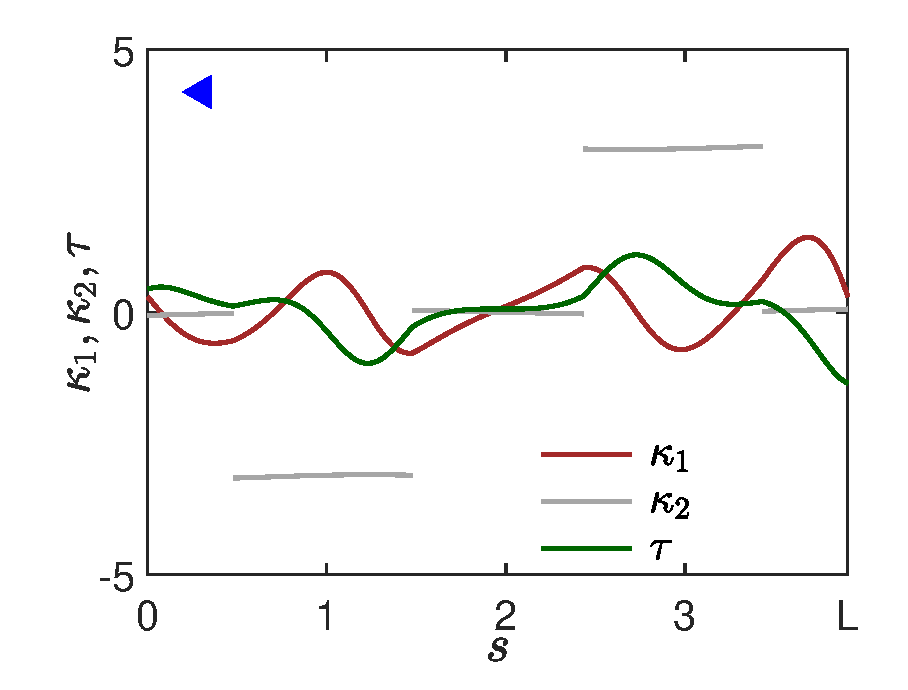
\includegraphics[width=0.45\linewidth]{Re.eps}}
	\subcaptionbox{~\Rlefttriangle~:$\kappa_1,\kappa_2,\tau$曲线\label{fig:Rf}}
	{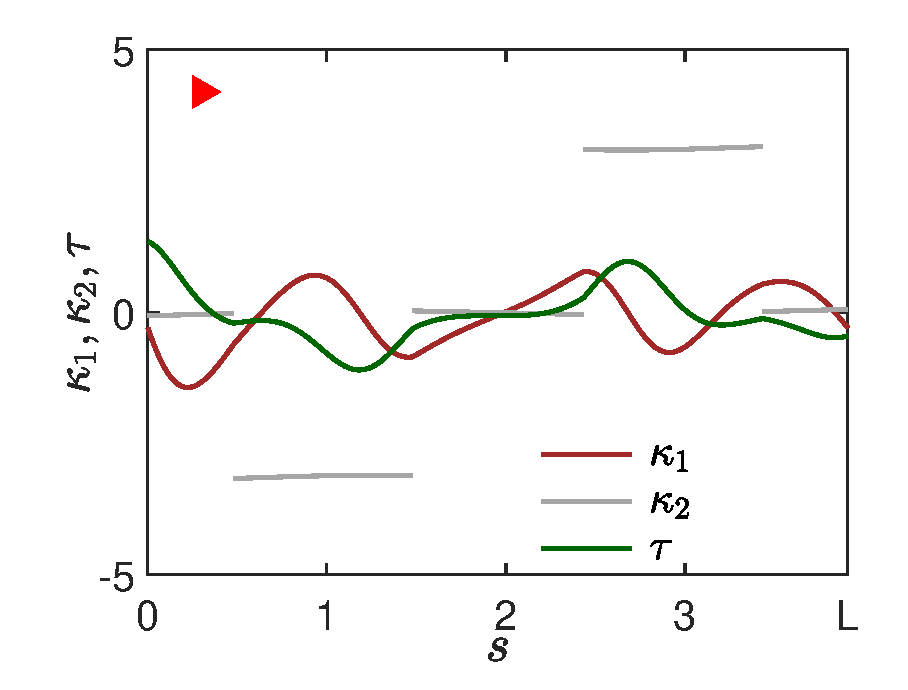
\includegraphics[width=0.45\linewidth]{Rf.eps}}\\
	\subcaptionbox{~\Brighttriangle~:$N_1,N_2,N_3$曲线\label{fig:Ri}}
	{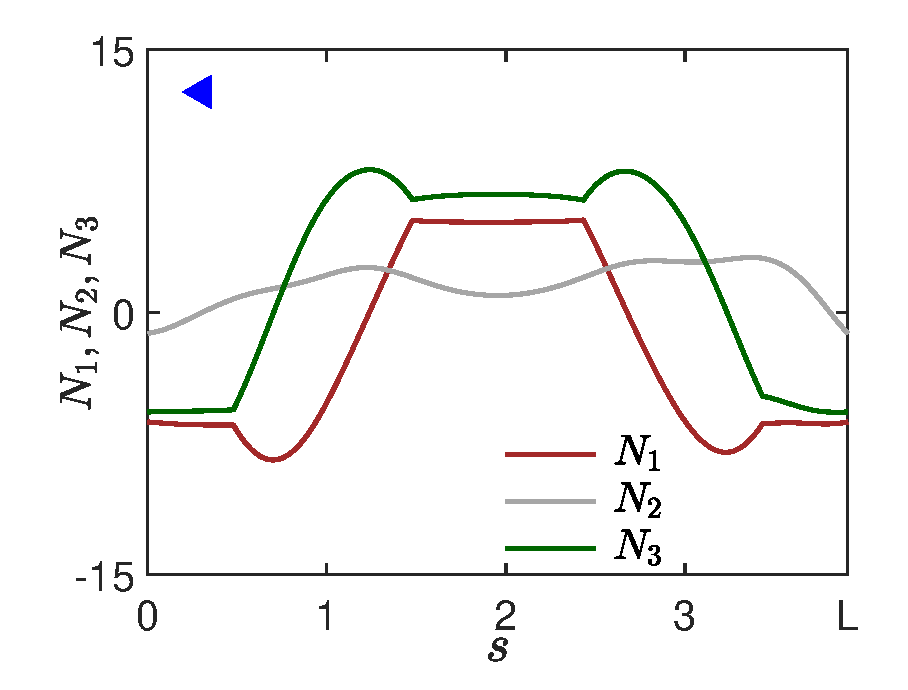
\includegraphics[width=0.45\linewidth]{Ri.eps}}
	\subcaptionbox{~\Rlefttriangle~:$N_1,N_2,N_3$曲线 \label{fig:Rj}}
	{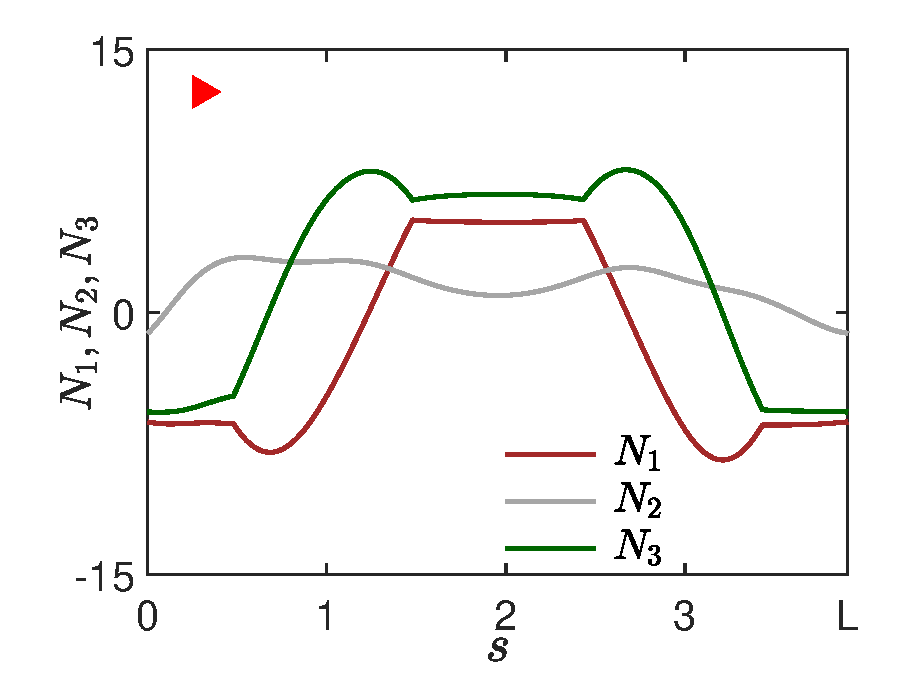
\includegraphics[width=0.45\linewidth]{Rj.eps}}
	\subcaptionbox{~\Blefttriangle~:$\kappa_1,\kappa_2,\tau$曲线\label{fig:Rg}}
	{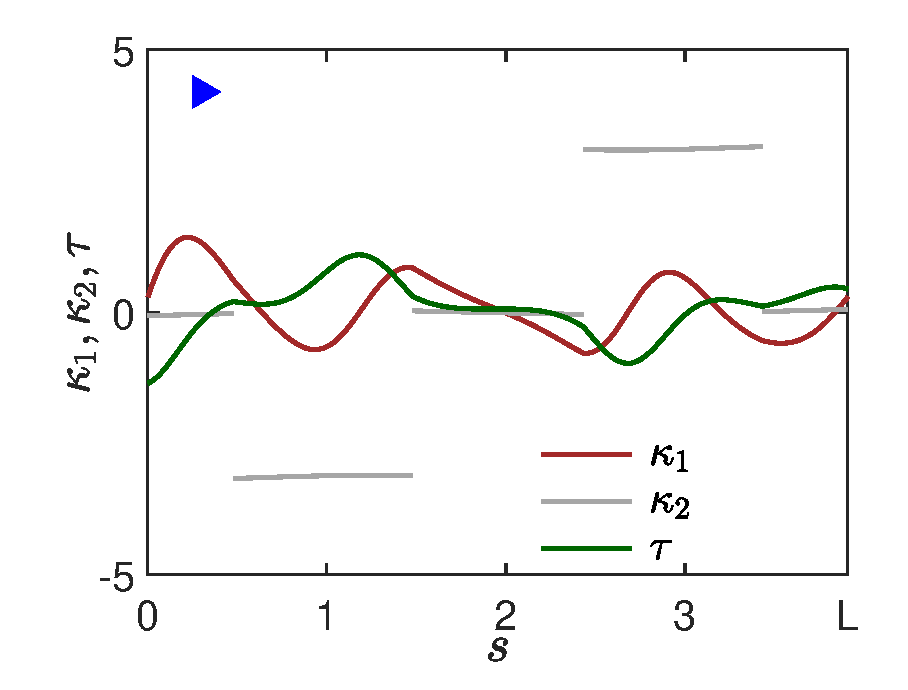
\includegraphics[width=0.45\linewidth]{Rg.eps}}
	\subcaptionbox{~\Rrighttriangle~:$\kappa_1,\kappa_2,\tau$曲线\label{fig:Rh}}
	{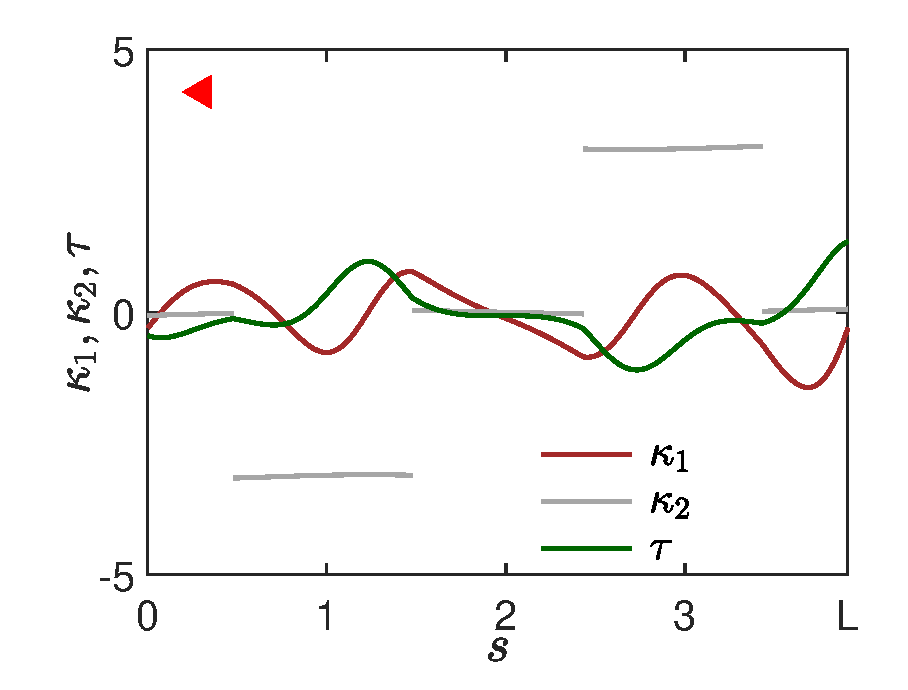
\includegraphics[width=0.45\linewidth]{Rh.eps}}\\
	\subcaptionbox{~\Blefttriangle~:$N_1,N_2,N_3$曲线\label{fig:Rk}}
	{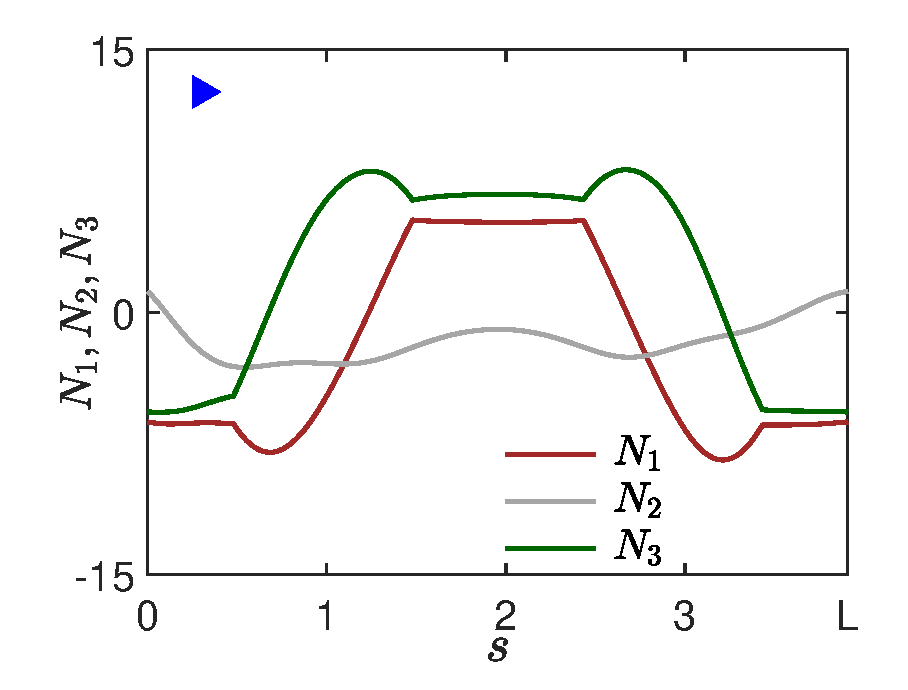
\includegraphics[width=0.45\linewidth]{Rk.eps}}
	\subcaptionbox{~\Rrighttriangle~:$N_1,N_2,N_3$曲线 \label{fig:Rl}}
	{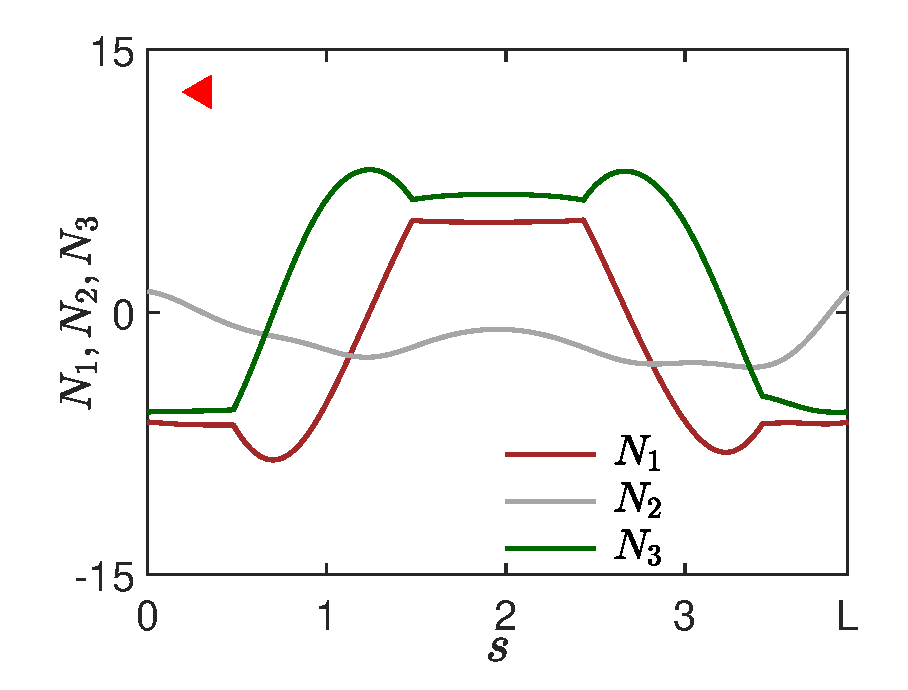
\includegraphics[width=0.45\linewidth]{Rl.eps}}
	\caption{图~\ref{fig:SerpentineNc1Aniso10}(c)中标记所对应的构形的解曲线}
	\label{fig:relation in reversible group}
\end{figure}
图~\ref{fig:relation in reversible group}为$\alpha=1.5$,$n_c=1$的蛇形结构的同一平衡构形组中的四个构形相应的解曲线,通过观察可知这六个变量具有如下关系:
\begin{equation}
	\begin{gathered}
		R_{1}: s \rightarrow L-s, \kappa_{20} \rightarrow-\kappa_{20}, \kappa_{1} \rightarrow-\kappa_{1}, \kappa_{2} \rightarrow-\kappa_{2}, \tau \rightarrow-\tau, N_{1} \rightarrow N_{1}, N_{2} \rightarrow N_{2}, N_{3} \rightarrow N_{3} \\
		R_{2}: s \rightarrow L-s, \kappa_{20} \rightarrow-\kappa_{20}, \kappa_{1} \rightarrow \kappa_{1}, \kappa_{2} \rightarrow-\kappa_{2}, \tau \rightarrow \tau, N_{1} \rightarrow N_{1}, N_{2} \rightarrow-N_{2}, N_{3} \rightarrow N_{3} \\
	\end{gathered}
	\label{eq:R1R2}
\end{equation}
将上述关系式带入原方程,可验证原方程形式保持不变,证明该关系具有普适性。若已知一平衡构形组中的一个解,则可以通过式\eqref{eq:R1R2}得到其余构形的解。例如,若第一个构形~\Brighttriangle~已知,那么通过关系式\eqref{eq:R1R2}中$R_1$变换可以得到第二个构形~\Rlefttriangle~相应的解。将第一个构形通过关系式\eqref{eq:R1R2}中$R_2$变换,可以得到构形~\Blefttriangle~对应的解。对于最后一个构形~\Rrighttriangle~,可以对第一个构形进行式\eqref{eq:K}中的$K$变换得到。最后,本处给出关于图~\ref{fig:relation in reversible pair}和图~\ref{fig:relation in reversible group}中$\kappa_2$不连续的原因:在半圆弧与直线段连接处,初始曲率$\kappa_{20}$不连续。
\subsection{蛇形条带的多稳态构形}
本小节给出单元数$n_c=1,2,3$的蛇形结构的稳态构形的数值计算结果以及相应的实验结果。本文首先通过实验观察到某一构形,随后观察可能的施加扰动方法,即通过在哪几个半圆弧端部施加扰动外力,可以从某一已知构形一步步切换到目标构形。然后利用离散弹性杆模型进行相应的动力学模拟来得到数值计算结果。利用该方法可以找到绝大多数稳态构形,但该方法依赖实验来寻找适合的外力类型,另外该方法无法保证可以找到所有稳态构形,即无法找到能量函数的所有局部最小值。因此,本节所列结果只是部分稳态构形,无法保证找到了所有稳定构形。
\begin{figure}[t]
	\centering
	\includegraphics[width=1\linewidth]{ExptsvsSimulations.pdf}
	\caption{不同单元数$n_c$,不同高度$\alpha$的蛇形条带在不同拉伸位移$D_x/H$下,稳定构形的二维俯视图($x-y$平面投影)。黑色背景中构形为实验结果,白色背景对应数值计算结果。(a-f) 单元数$n_c=1$,$\alpha=1.5$的蛇形结构。(g-k) 单元数$n_c=1$,$\alpha=4$的蛇形结构。(l-p) 单元数$n_c$=2,高度$\alpha=3$的蛇形结构。(q-z)单元数$n_c$=3,高度$\alpha=3$的蛇形结构。在每个子图下面$m_n$代表一组$m$个蛇形结构中的$n$个构形}
	\label{fig:ExptsvsSimulations}
\end{figure}

图~\ref{fig:ExptsvsSimulations}展示了不同单元数$n_c$,不同高度$\alpha$的蛇形条带在水平拉伸位移$D_x/H$下的稳定构形的$x-y$方向投影,其中黑色背景为实验结果而白色背景中构形为相应的数值计算结果。在每一个子图下面,用$m_n$代表该构形为一组$m$个构形中的第$n$个构形(顺序$n$为随机排列)。

对于单单元蛇形结构,图~\ref{fig:ExptsvsSimulations}(b-d),(f),(h-j)中的构形表现出了自可逆性(self-reversibility),每一构形为所属自可逆构形对中的一个构形。图~\ref{fig:ExptsvsSimulations}($j_1$),($j_2$)给出了一个自可逆构形对的所有构形。而图~\ref{fig:ExptsvsSimulations}(a),(e),(g),(k)中构形并没有自可逆性,每一个构形均为相应平衡构形组中的一个构形。

对于$\alpha=1.5$,$n_c=1$的蛇形结构,图~\ref{fig:ExptsvsSimulations}(a)对应图~\ref{fig:SerpentineNc1Aniso10}(a)中~\Brighttriangle~所标记的分支;图~\ref{fig:ExptsvsSimulations}(b)中构形为S模态,对应图~\ref{fig:SerpentineNc1Aniso10}(a)中~\bluesquare~所标记的分支;图~\ref{fig:ExptsvsSimulations}(c)为M模态,对应图~\ref{fig:SerpentineNc1Aniso10}(a)中~\Btriangle~所标记的分支;图~\ref{fig:ExptsvsSimulations}(d)对应图~\ref{fig:SerpentineNc1Aniso10}(a)中~\Bdiamond~所标记的分支;图~\ref{fig:ExptsvsSimulations}(e)对应图~\ref{fig:SerpentineNc1Aniso10}(a)中~\HBrighttriangle~所标记的分支;图~\ref{fig:ExptsvsSimulations}(f)对应图~\ref{fig:SerpentineNc1Aniso10}(a)中~\Bstarshape~所标记的分支。

对于$\alpha=4$,$n_c=1$的蛇形结构。图~\ref{fig:ExptsvsSimulations}(g)对应图~\ref{fig:SerpentineNc1Aniso10}(d)中~\Brighttriangle~所标记的分支;图~\ref{fig:ExptsvsSimulations}(h)对应图~\ref{fig:SerpentineNc1Aniso10}(d)中~\Bdiamond~所标记的分支;图~\ref{fig:ExptsvsSimulations}(i)中构形为S模态,对应图~\ref{fig:SerpentineNc1Aniso10}(d)中~\bluesquare~所标记的分支;图~\ref{fig:ExptsvsSimulations}($j_1$),($J_2$)为M模态,对应图~\ref{fig:SerpentineNc1Aniso10}(d)中~\Btriangle~/~\Rtriangle~所标记的分支;图~\ref{fig:ExptsvsSimulations}(k)对应图~\ref{fig:SerpentineNc1Aniso10}(d)中~\HBrighttriangle~所标记的分支。

随着单元的增多,稳态个数及相应的分支曲线也会增多,为了保证分岔图的清晰性,尽管在图~\ref{fig:ExptsvsSimulations}中展示了许多稳态,但多单元蛇形条带分岔图~\ref{fig:SerpentineNc2Nc3Aniso10Phase}并未将这些稳态对应的分岔曲线一一展示。图~\ref{fig:ExptsvsSimulations}(l-p)展示了$(n_c,\alpha)=(2,3)$的蛇形结构在拉伸载荷下的部分稳定构形。图~\ref{fig:ExptsvsSimulations}(l),(m)为自可逆构形,分别对应S模态和M模态。图~\ref{fig:ExptsvsSimulations}($n_1$),($n_2$)为一自可逆构形对。图~\ref{fig:ExptsvsSimulations}($o_1$),($o_2$),($o_3$),($o_4$)给出了同一平衡构形组中的所有构形,而图~\ref{fig:ExptsvsSimulations}($p_1$),($p_2$)为另一个平衡构形组中的其中两个构形。因此,对于$n_c=2$的蛇形条带,本文找到了14个平衡构形。

图~\ref{fig:ExptsvsSimulations}(q-z)展示了$(n_c,\alpha)=(3,3)$的蛇形结构在拉伸载荷下的部分稳定构形。每一构形都属于不同的自可逆构形对或者平衡构形组。其中,图~\ref{fig:ExptsvsSimulations}(q),(r),(v),(w)中的构形分别属于不同的自可逆构形对,其中图~\ref{fig:ExptsvsSimulations}(q)为S模态,图~\ref{fig:ExptsvsSimulations}(r)为M模态。其余的构形分别属于不同的平衡构形组。因此,对于$(n_c,\alpha)=(3,3)$的蛇形结构,这里识别了三十二个平衡构形。

从图~\ref{fig:ExptsvsSimulations}可以看到数值计算的构形与实验结果吻合良好,进一步说明了本文所用计算模型对该结构的有效性,以及实验装置的精确性。

%模板中使用 \pkg{unicode-math} 宏包来配置数学符号,
%
%研究生《写作指南》要求量及其单位所使用的符号应符合国家标准《国际单位制及其应用》(GB 3100—1993)、《有关量、单位和符号的一般原则》(GB/T 3101—1993)的规定,但是与 \TeX{} 默认的美国数学学会(AMS)的符号习惯有所区别。
%
%英文论文的数学符号使用 \TeX{} 默认的样式。论文以中文为主要撰写语言按照国标建议的配置数学字体格式:
%
%\begin{enumerate}
%  \item 大写希腊字母默认为斜体,如
%    \begin{equation*}
%      \Gamma \Delta \Theta \Lambda \Xi \Pi \Sigma \Upsilon \Phi \Psi \Omega.
%    \end{equation*}
%    注意有限增量符号 $\increment$ 固定使用正体,模板提供了 \cs{increment} 命令。
%  \item 小于等于号和大于等于号使用倾斜的字形 $\le$、$\ge$。
%  \item 积分号使用正体,比如 $\int$、$\oint$。
%  \item 行间公式积分号的上下限位于积分号的上下两端,比如
%    \begin{equation*}
%      \int_a^b f(x) \dif x.
%    \end{equation*}
%    行内公式为了版面的美观,统一居右侧,如 $\int_a^b f(x) \dif x$ 。
%  \item
%    偏微分符号 $\partial$ 使用正体。
%  \item
%    省略号 \cs{dots} 按照中文的习惯固定居中,比如
%    \begin{equation*}
%      1, 2, \dots, n \quad 1 + 2 + \dots + n.
%    \end{equation*}
%  \item
%    实部 $\Re$ 和虚部 $\Im$ 的字体使用罗马体。
%\end{enumerate}
%%
%%以上数学符号样式的差异可以在模板中统一设置。
%%另外国标还有一些与 AMS 不同的符号使用习惯,需要用户在写作时进行处理:
%\begin{enumerate}
%  \item 数学常数和特殊函数名用正体,如
%    \begin{equation*}
%      \uppi = 3.14\dots; \quad
%      \symup{i}^2 = -1; \quad
%      \symup{e} = \lim_{n \to \infty} \left( 1 + \frac{1}{n} \right)^n.
%    \end{equation*}
%  \item 微分号使用正体,比如 $\dif y / \dif x$。
%  \item 向量、矩阵和张量用粗斜体(\cs{mathbfit}),如 $\mathbfit{x}$、$\mathbfit{\Sigma}$、$\mathbfit{T}$。
%  \item 自然对数用 $\ln x$ 不用 $\log x$。
%\end{enumerate}
%
%
%
%关于数学符号更多的用法,参考
%\href{http://mirrors.ctan.org/macros/latex/contrib/unicode-math/unicode-math.pdf}{\pkg{unicode-math}}
%宏包的使用说明,
%全部数学符号命的令参考
%\href{http://mirrors.ctan.org/macros/latex/contrib/unicode-math/unimath-symbols.pdf}{\pkg{unimath-symbols}},也可以参考 Stack Overflow 上的答案 \href{https://tex.stackexchange.com/questions/58098/what-are-all-the-font-styles-i-can-use-in-math-mode}{What are all the font styles I can use in math mode?}。
%
%关于量和单位推荐使用
%\href{http://mirrors.ctan.org/macros/latex/contrib/siunitx/siunitx.pdf}{\pkg{siunitx}}
%宏包,
%可以方便地处理希腊字母以及数字与单位之间的空白,
%比如:
%\SI{6.4e6}{m},
%\SI{9}{\micro\meter},
%\si{kg.m.s^{-1}},
%\SIrange{10}{20}{\degreeCelsius}。
%
%
%数学公式可以使用 \env{equation} 和 \env{equation*} 环境。
%注意数学公式的引用应前后带括号,建议使用 \cs{eqref} 命令,比如式\eqref{eq:example}。
%\begin{equation}
%  \frac{1}{2 \uppi \symup{i}} \int_\gamma f = \sum_{k=1}^m n(\gamma; a_k) \mathscr{R}(f; a_k)
%  \label{eq:example}
%\end{equation}
%注意公式编号的引用应含有圆括号,可以使用 \cs{eqref} 命令。
%
%晶体衍射基础的著名公式──布拉格方程:
%\begin{equation}
%  2d\sin\theta=k\lambda, \quad k=1,2,3\ldots
%\end{equation}
%
%\noindent%
%\begin{minipage}{\textwidth}
%  \begin{tabularx}{\textwidth}{@{}l@{~}l@{~——~}X@{}}
%    式中 & $d$ & 晶面间距(nm);\\
%    & $\theta$ & 入射线与晶面的夹角(rad);\\
%    & $\lambda$ & X射线波长(nm)。\\
%    & $k$ & 公式中第一次出现的物理量代号应给予注释,注释的转行应与破折号“——”后第一个字对齐。
%  \end{tabularx}
%\end{minipage}
%
%多行公式尽可能在“=”处对齐,推荐使用 \env{align} 环境。
%\begin{align}
%  a & = b + c + d + e \\
%    & = f + g
%\end{align}
%
%此外需要注意:公式需紧挨段前文字,不可空行,不然会导致公式独立成段,如下\textcolor{red}{\textbf{错误}}效果。公式前文字公式前文字公式前文字公式前文字公式前文字。
%
%\begin{equation}
%  \frac{1}{2 \uppi \symup{i}} \int_\gamma f = \sum_{k=1}^m n(\gamma; a_k) \mathscr{R}(f; a_k)
%\end{equation}
%
%公式后文字公式后文字公式后文字公式后文字公式后文字公式后文字公式后文字公式后文字公式后文字公式后文字公式后文字。\textbf{正确}效果,如下:
%% <- 如需代码上空行需要在前面加上百分号·%
%\begin{equation}
%  \frac{1}{2 \uppi \symup{i}} \int_\gamma f = \sum_{k=1}^m n(\gamma; a_k) \mathscr{R}(f; a_k)
%\end{equation}
%公式后文字公式后文字公式后文字公式后文字公式后文字公式后文字公式后。
%
%\section{数学定理}
%
%定理环境的格式可以使用 \pkg{amsthm} 或者 \pkg{ntheorem} 宏包配置。
%用户在导言区载入这两者之一后,模板会自动配置 \env{thoerem}、\env{proof} 等环境。
%
%\begin{theorem}[Lindeberg--Lévy 中心极限定理]
%  设随机变量 $X_1, X_2, \dots, X_n$ 独立同分布, 且具有期望 $\mu$ 和有限的方差 $\sigma^2 \ne 0$,
%  记 $\bar{X}_n = \frac{1}{n} \sum_{i+1}^n X_i$,则
%  \begin{equation}
%    \lim_{n \to \infty} P \left(\frac{\sqrt{n} \left( \bar{X}_n - \mu \right)}{\sigma} \le z \right) = \Phi(z),
%  \end{equation}
%  其中 $\Phi(z)$ 是标准正态分布的分布函数。
%\end{theorem}
%\begin{proof}
%  Trivial.
%\end{proof}
%
%同时模板还提供了 \env{assumption}、\env{definition}、\env{proposition}、
%\env{lemma}、\env{theorem}、\env{axiom}、\env{corollary}、\env{exercise}、
%\env{example}、\env{remar}、\env{problem}、\env{conjecture} 这些相关的环境。
%
%\section{数学字体}
%
%按照《撰写规范》表达式字体可以采用 Times New Roman、Xits Math 或 Cambria Math(MS Word默认字体)。Cambria Math 缺少部分样式,例如:积分符号设定为 upright 也看起来没有变化。
%
%TeX Gyre Termes Math 字体(Times New Roman的TeX克隆版)样例:
%\makeatletter
%\thu@load@math@font@times
%\begin{equation}
%  \frac{1}{2 \uppi \symup{i}} \int_\gamma f = \sum_{k=1}^m n(\gamma; a_k) \mathscr{R}(f; a_k)
%\end{equation}
%\makeatother
%
%Cambria Math 字体样例:
%\makeatletter
%\thu@load@math@font@cambria
%\begin{equation}
%  \frac{1}{2 \uppi \symup{i}} \int_\gamma f = \sum_{k=1}^m n(\gamma; a_k) \mathscr{R}(f; a_k)
%\end{equation}
%\makeatother
%
%Xits Math 字体样例:
%\makeatletter
%\thu@load@math@font@xits
%\begin{equation}
%  \frac{1}{2 \uppi \symup{i}} \int_\gamma f = \sum_{k=1}^m n(\gamma; a_k) \mathscr{R}(f; a_k)
%\end{equation}
%\thu@load@math@font@cambria
%\makeatother
%
%STIX Math 字体样例:
%\makeatletter
%\thu@load@math@font@stix
%\begin{equation}
%  \frac{1}{2 \uppi \symup{i}} \int_\gamma f = \sum_{k=1}^m n(\gamma; a_k) \mathscr{R}(f; a_k)
%\end{equation}
%\makeatother

